\setTopic{Sets and Functions}
\setAuthor{M. Andrew Moshier}
\setDate{October 2014}
\setCourse{Discrete Mathematics}

\setOverview{
The mathematical universe consists of various things: numbers, functions, graphs, lists and so on.
A \noexpand\emph{set} is a collection of things. 
For example, the collection of all natural numbers is a set.
A \noexpand\emph{function} is a correlation of the members of one set with members of another set.
These two abstract concepts (sets and functions) form a conceptual framework in which virtually all of mathematics can be built.
So an understanding of sets and functions is key to a rigorous approach to most other parts of mathematics.
This conceptual framework can itself be put on a formal, precise footing called the Category of Sets and Functions.

In these lectures, we build up the Category of Sets and Functions, so that we can use these things as the basic building blocks of everything else we do.
}

\chapter{Sets}

\begin{goals}
\noindent\textbf{Lecture}
\begin{itemize}
\item Describe informally the category of sets.
\item Define list set notation.
\item Introduce the idea of a subset.
\item Introduce the axiom of extensionality for sets and some of its consequences.
\end{itemize}

\noindent\textbf{Study}
\begin{itemize}
\item Demonstrate ability to determine equality of sets.
\item Develop facility in basic set theoretic notation.
\end{itemize}
\end{goals}

\emph{Sets} are the mathematician's way of thinking about \emph{collections} of objects. Examples will be the set of natural numbers, the set of pairs of natural numbers, the set of lists of natural numbers, and so on.
\emph{Functions} are the mathematicians way of thinking about operations, such as successor, addition, summation, and so on.

Mathematicians also use functions to model attributes of the things in a collection, like ``the color of'', ``the mass of'', ``the location of'', ``the father of'', ``the favorite book of the person to the left of'' and so on.
There is little sense in saying these are ``operations'', but they have a similar behavior. For each potential
object $x$ of the right sort (a wooden building block, for example), \emph{the color of $x$} is a specific color. Similarly,
for a natural number $n$, ``the successor of $n$'' is another specific natural number. So ``the color of'' is a function
from the set of wooden building blocks to the set of colors; ``the successor of''
is a function from the set of natural numbers to set of natural numbers. Likewise, addition constitutes a function from the set of 
pairs of natural numbers to the set of natural numbers. In English we might say ``the sum of $m$ and $n$'', but we usually write $m+n$. 
Either way, any pair of natural numbers has a sum. So ``the sum of'' is an attribute of pairs of natural numbers, just like ``the color of'' is an attribute of wooden building blocks.

Taken together, sets and functions constitute a fundamental structure in contemporary mathematics called the \emph{Category of Sets and Functions}. 
This is a slight lie.
Actually, there are many different categories of sets that differ in subtle ways. 
But for most mathematics, the differences are irrelevant.
So in practice, it is safe to talk as if there is just one category of sets.
The Category of Sets and Functions sometimes abbreviated as \textbf{Set}.

To understand sets and functions as they are used in every day mathematics, we need to answer some questions:
\begin{itemize}
	\item What do we mean by saying that a set is a collection?
	\item What do we mean by saying that two sets are equal?
	\item What do we mean by saying that a function behaves like an attribute?
	\item What do we mean by saying that two functions are equal?
\end{itemize}
The answers to these leads to some basic principles for reasoning about sets and functions. 
Other principles allow us to construct sets and functions with specific behaviors. 
We could be more formal and present these principles as \emph{axioms}, but the word ``axiom''
has a special connotation in mathematics that we do not need here. Nevertheless, everything we say in these lectures could be presented in terms of formal axioms.  

\section{Set Basics}

A set consists of things that are ``in'' the set. All other things are ``not in'' the set. 
For example, later we will see that the natural numbers constitute a set $\NN$. 
So $0$ is in $\NN$, $1$ is in $\NN$, and so on, but $\frac{1}2$ is not in $\NN$.
We make this precise and introduce notation for the idea.

\begin{signature}\label{sig:SetSignature}
  A \emph{set} is a mathematical entity $A$ with the following feature. 
  For any thing $x$, either $x$ \emph{is in} $A$ or $x$ \emph{is not in} $A$. 
  We write $x\in A$ if $x$ is in $A$ and $x\notin A$ if $x$ is not in $A$.

The symbol $\in$ is used in mathematics exclusively to indicate membership in a set. 
You will not see it used in any other way.  

For variety, all of the following phrases mean the same thing:
\begin{itemize}
\item $x$ is in $A$
\item $x$ is an \emph{element of} $A$
\item $x$  is a \emph{member of} $A$
\item $A$ \emph{contains} $x$
\item $x$ \emph{belongs to} $A$
\end{itemize}
\end{signature}

Basic Vocabulary \ref{sig:SetSignature} describes how we can talk about sets and elements, and how to use the notation of membership, but does not tell us that any sets actually exist. 
We will remedy that in the next sections.
Our first remedy is to make room for finite sets.

\begin{principle}[Finite Sets] For any list $L  = [a_0,\ldots, a_{n-1}]$, there is a set, denoted by $\{a_0,\ldots,a_{n-1}\}$, so
  that $x\in \{a_0,\ldots, a_{n-1}\}$ if and only if $x=a_i$ for some
  $i<n$.  More precisely,
  \begin{itemize}
  \item $x\notin \{\}$ for any $x$ (so $\{\}$ is said to be \emph{empty});
  \item $x\in \{a_0,\ldots,a_n\}$ if and only if $x=a_0$ or $x\in
    \{a_1,\ldots,a_n\}$.
  \end{itemize}
\end{principle}

\printbreak

\begin{example}
Here are some examples of sets built from finite lists:
\begin{itemize}
\item $\{\}$ -- an empty set;
\item $\{1,2,5\}$ -- a set consisting of three elements;
\item $\{\{\}\}$ -- a set consisting of one element, which is $\{\}$;
\item $\{1,2,4,\{1,2\}\}$ -- a set consisting of four elements, $1$,
  $2$, $4$ and the set $\{1,2\}$.
\item $\{4,5, \{\}, [\,]\}$ -- a set consisting of four elements. Note that
the set $\{\}$ and the list $[\,]$ are not the same things.
\item $\{1,2,3,4,3,2,1\}$ -- a set consisting of four elements, listing an element twice is redundant.
\end{itemize}
\end{example}

The study of finite sets is surprisingly complex, and comprises a large part of
the branch of mathematics called \emph{combinatorics}. We will touch on some basics
of combinatorics later in the course. 

Various infinite sets of numbers also exist. All of these are indeed sets (that is, their existence follows from general principles
of set theory), but we will not try to justify that explicitly, except for the set of natural numbers.

\begin{defn}
	The following sets are denoted by special symbols:
	\begin{align*}
		\NN &= \text{the set of natural numbers}\\
		\ZZ &= \text{the set of integers}\\
		\QQ &= \text{the set of rational numbers}\\
		\RR &= \text{the set of real numbers}\\
		\CC &= \text{the set of complex numbers}
	\end{align*}
\end{defn}


\begin{exercises}
	\begin{enumerate}
  \item Let $A = \{1,\{2,3\},4\}$. Determine which of the following assertions are true.
    \begin{enumerate}
    \item $1\in A$
    \item $2\in A$
    \item $\{\}\in A$
    \item $\{2,3\}\in A$
    \item $A\in A$
    \end{enumerate}
  \item In the following examples of sets with elements following a pattern, write an expression for the same set
  that makes the pattern clearer.
  \begin{enumerate}
  \item $\{0,2,4,\ldots, 100\}$
  \item $\{1,2,4,8,\ldots, 256\}$
  \item $\{0,1,3, 6, 10,\ldots, 55\}$
  \end{enumerate}
  \end{enumerate}
\end{exercises}

\section{Subsets and Extensionality}

Sets are meant to be bare collections. For a set $A$, some things are in $A$, some are not. And that's all we can say.
Unlike a list, a set has no ``initial'' element.
For example, the set $\{1,2,3\}$ should be the same as the set $\{2,3,1\}$, because both have the same elements. This is an important difference between
lists and sets: $[1,2,3]$ and $[2,3,1]$ are \emph{not} the same lists because order matters in lists. 
To make this precise, we need to be clear about when sets are equal. To do this, we introduce an important definition.

\begin{defn}
  For sets $A$ and $B$, we say that \emph{$A$ is a subset of $B$} provided that every element of $A$ is an element of $B$. We also
  write this as $A\subseteq B$, and say that \emph{$A$ is included in $B$}.  We may also write $B\supseteq A$ 
  to mean the same thing, and say that \emph{$B$ is a superset of $A$}.

  If $A$ is \emph{not} a subset of $B$, we write $A\not\subseteq B$. If $A\subseteq B$ and $B\not\subseteq A$, then $A$ is called a
  \emph{proper subset of $B$}. To indicate that $A$ is a \emph{proper} subset of $B$, we may write $A\subsetneq B$.
\end{defn}

Saying $A\subseteq B$ is exactly the same as saying that for any $x$, if $x\in A$ then $x\in B$.

\begin{example}
  Here are some examples and counter-examples of the subset relation.
  \begin{itemize}
  \item $\{1,2,3\}\subseteq \{0,1,2,3\}$
  \item $\{\}\subseteq \{0\}$
  \item $A\subseteq A$ for any set $A$ because, trivially, every
    element of $A$ is an element of $A$
  \item $\{\} \subseteq A$ for any set $A$ because every element of
    $\{\}$ (there are none) is an element of $A$
  \item $\{1,2,3\}\not\subseteq \{0,2,3\}$ because $1\in \{1,2,3\}$
    but $1\notin \{0,2,3\}$
  \item $\{1,2,3\}\subseteq \{2,3,1\}$
  \end{itemize}
\end{example}

\ipadbreak

\begin{exercises}
	For each of the following pairs of sets, determine whether or
  not the first is a subset of the second. Explain your answer.
  \begin{enumerate}[series=exercises]
  \item $\{0,1\}$ and $\{1,0\}$
  \item $\{a,b,c,d\}$ and $\{a,b,d,e,c\}$
  \item $\{\}$ and $\{\{\}\}$
  \item $\{0,3,6,10\}$ and $\{10,9,8,7,6,5,4,2,1, 0\}$
  \end{enumerate}
\end{exercises}


We can summarize two useful properties of $\subseteq$ as follows.
\begin{itemize}
	\item{}[Reflexivity]  For any set $A$, $A \subseteq A$. We say $\subseteq$ is \emph{reflexive}.
	\item{}[Transitivity] For any sets $A$, $B$ and $C$,
	if $A\subseteq B$ and $B\subseteq C$, then $A\subseteq C$. We say $\subseteq$ is \emph{transitive}.
\end{itemize}
Another familiar example of a reflexive, transitive
relation is $\leq$ on the natural numbers. In fact there are many examples of reflexive transitive relations throughout mathematics. 

The relation $\leq$ is also \emph{anti-symmetric}, meaning that if $m\leq n$ and $n\leq m$ then $m=n$. 
Suppose $A\subseteq B$ and $B\subseteq A$. Then, by definition $A$ and $B$ have the exact same elements.  By our understanding of sets as collections,
$A$ and $B$ must be equal. So we state this as another axiom.

\begin{principle}\label{ax:set-extensionality}
[\textbf{The Axiom of Set Extensionality}]
For sets $A$ and $B$, if $A\subseteq B$ and $B\subseteq A$, then $A=B$. In other words, $\subseteq$ is anti-symmetric.
\end{principle}

Based on this, we can already establish a useful fact: there is exactly one empty set. To set the tone for what follows, we make this a formal claim.

\begin{lemma}
	There is exactly one empty set.
\begin{proof}
	We have already noted that the set built from an empty list $\{\,\}$ has no elements. So there is at least one empty set.
	
	Suppose $E$ is a set with no elements.
	Then $E\subseteq \{\,\}$ because every element of $E$ (there are none) is an element of $\{\,\}$. 
	Similarly, $\{\,\}\subseteq E$ because every element of $\{\,\}$ (again, there are none) is an element of $E$. 
	So by Principle~\ref{ax:set-extensionality} $E = \{\,\}$.
\end{proof}
\end{lemma}

\begin{defn}
  The set $\{\}$ is also denoted by $\emptyset$.
\end{defn}

Set extensionality makes precise the idea that a set by itself does
not have any structure other than what members it possesses.
To emphasize this, sometimes it is useful to
depict a set with elements scattered about something like \usetikzlibrary{fit,shapes}
\[\begin{tikzpicture}[ >=stealth, bullet/.style={ fill=black, circle,
    minimum width=1pt, inner sep=2pt }, projection/.style={ ->, thick,
    shorten <=2pt, shorten >=2pt }, every fit/.style={ ellipse, draw,
    inner sep=2pt } ]
  \foreach \x/\y/\l in {0.4/1/d,-0.2/2/c/,0/3/b,0.5/4/a}
  \node[bullet,label=left:$\l$] (a\y) at (\y,\x) {};
  \node[draw,fit=(a1) (a2) (a3) (a4),minimum width=2cm] {} ;
\end{tikzpicture}
\]
with the elements scattered about. Evidently, a re-arrangement of the
elements does not change the depicted set. So
\[\usetikzlibrary{fit,shapes}
\begin{tikzpicture}[ >=stealth, bullet/.style={ fill=black, circle,
    minimum width=1pt, inner sep=2pt }, projection/.style={ ->, thick,
    shorten <=2pt, shorten >=2pt }, every fit/.style={ ellipse, draw,
    inner sep=2pt } ]
  \foreach \x/\y/\l in {0.3/2/d,-0.2/3/c/,0/4/b,-0.5/1/a}
  \node[bullet,label=left:$\l$] (a\y) at (\y,\x) {};
  \node[draw,fit=(a1) (a2) (a3) (a4),minimum width=2cm] {} ;

\end{tikzpicture}
\]
is the same set. Depicting a subset of a set is a simple
matter of drawing a smaller boundary around some of the elements as in the following.
\[\usetikzlibrary{fit,shapes}
\begin{tikzpicture}[ >=stealth, bullet/.style={ fill=black, circle,
    minimum width=1pt, inner sep=2pt }, projection/.style={ ->, thick,
    shorten <=2pt, shorten >=2pt }, every fit/.style={ ellipse, draw,
    inner sep=2pt } ]
  \foreach \x/\y/\l in {0.3/2/d,-0.2/3/c/,0/4/b,-0.5/1/a}
  \node[bullet,label=left:$\l$] (a\y) at (\y,\x) {};
  \node[draw,fit=(a1) (a2) (a3) (a4),minimum width=2cm] {} ;
  \node[draw, fit = (a2) (a3), minimum width=2cm] {};
\end{tikzpicture}
\]
\ipadbreak

\begin{exercises}
Draw depictions of the following sets
  \begin{enumerate}[resume=exercises]
  \item $\{1,4,5,2,3\}$
  \item $\{1,2,3,\ldots, 23\}$
  \item $\{a,b,c,d,e\}$ and $\{c,e,f,g\}$ on the same diagram
  \item $\{a, e, b,c,e\}$ [sic]
  \item $\{1,3,6,7\}$ and $\{1,3,5,6,7,9\}$ on the same diagram
  \item $\{\bot,\top$
  \item $\{\bullet\}$
  \item $\{\top,\bot,3,5,1, \bullet\}$
  \end{enumerate}
\end{exercises}

\chapter{Functions}

\begin{goals}
\noindent\textbf{Lecture}
\begin{itemize}
\item Introduce basic structure of functions
\item Define the identity functions and function composition
\item Introduce internal diagrams of functions.
\end{itemize}

\noindent\textbf{Study}
\begin{itemize}
\item Be able to determine equality of functions
\item Use internal diagrams to depict function composition
\end{itemize}
\end{goals}

\emph{Functions} (perhaps in your calculus courses) are often talked about as \emph{operations}. 
For example, 
\[f(x) = x^2-1\]
can be seen as an operation that transforms a number $x$ into its square.
But it can also be seen as an attribute (the ``square of $x$'').
The ``operational'' view is informal, and often useful.
As we will see, though, it gets an important aspect of functions wrong because two entirely different operations may define the same function.

Informally, a function ``takes'' an argument from a given set as input and ``produces'' an output in a given set.
So the function $f$ defined by $f(x)=x^2 + 2x + 1$ might ``take'' the natural number $2$ and ``produce'' the natural number $10$. 
That is, $f(3)=3^2 + 1 = 10$. 
We begin by introducing the vocabulary of functions.

\begin{signature}
	\begin{itemize}
	\item For a set $A$ and a set $B$, there are things called \emph{functions from $A$ to $B$}, with a function $f$ from $A$ to $B$ being writing $\fromto fAB$ or $A\stackrel{f}{\to} B$. 

	\item For $\fromto fAB$, the set $A$ is called the \emph{domain} of $f$ and $B$ is called the \emph{codomain} of $f$.
	
	\item For any function $\fromto fAB$ and every element $a\in A$, $f$ and $a$ determine an element of $B$, written $f(a)$, and read ``$f$ of $a$''.
	\end{itemize}
\end{signature}

A functions may sometimes also be called a \emph{map}, a \emph{transformation}, or an \emph{operation}. 
As we will see, however, \emph{operation} is somewhat misleading. 

Often, a function $\fromto fAB$ is \emph{defined} by a rule, just as they are familiar in other parts of mathematics. 
We typically, write such rules by giving the function a name (very often $f$) and spelling out the rule at the same time.
So we write things like
\[f(x)=x^2 + 4x + 2\]
to define a function $\fromto f\RR\RR$ (recall that $\RR$ is the set of real numbers).
But sometimes it is useful to have a rule without giving it a name.
To do that, we use the ``maps to'' arrow $\mapsto$.
So we might define the same function $f$ by saying that \emph{$f$ is given by the rule $x\mapsto x^2 + 4x + 2$}. 
We will not go so far as to write $f = (x\mapsto x^2+4x+2)$ because this more easily understood by writing $f(x)=x^2+4x+2$.
The rule $x\mapsto x^2  4x + 2$ is the same as the rule $y\mapsto y^2 + 4y + 2$. 
The variable only serves as a place holder, so its particular name does not matter.

There are two fundamental (trivial) types of rules that can be used to build functions.

\begin{axiom}
	\begin{itemize}
		\item For any set $A$, there is a function $\fromto {\id_A}AA$ defined by the rule $x\mapsto x$.
		This is called the \emph{identity} function on $A$
		\item For any two functions $\fromto fAB$ and $\fromto gBC$, there is a function $\fromto {g\circ f}AC$ defined by the rule $x\mapsto g(f(x))$.
		This is called the composition of $g$ and $f$ (or sometimes ``$g$ following $f$'').
	\end{itemize}
\end{axiom}

Notice that $g\circ f$ is only defined when the \emph{domain} of $g$ matches the codomain of $f$.
Also, be careful about definitions like $f(x)=1/x$.
This does not define a function on the real numbers because $f(0)$ is undefined.
In other words, to be a function, $f$ must determine an element of the codomain for each element of the domain.

\begin{exercises}
Suppose $\fromto fAB$, $\fromto gBC$ and $\fromto hCD$ are functions. Then $h\circ(g\circ f)$ and $(h\circ g)\circ f$ are functions
from $A$ to $D$. Do you think they are equal? Explain your answer in a few clearly written sentences.	
\end{exercises}

\section{Internal Diagrams}

To depict a function on small sets, we can use the simple internal diagrams of the last section. For example,
\[
  \begin{tikzpicture}[
    >=stealth,
    bullet/.style={
      fill=black,
      circle,
      minimum width=1pt,
      inner sep=1pt
    },
    projection/.style={
      ->,
      thick,
      shorten <=2pt,
      shorten >=2pt
    },
    every fit/.style={
      ellipse,
      draw,
      inner sep=0pt
    }
  ]
    \foreach \x/\y/\l in {0.4/1/d,-0.2/2/c/,0/3/b,0.5/4/a}
      \node[bullet,label=left:$\l$] (a\y) at (\x,\y) {};

    \foreach \x/\y/\l in {4.1/1/4,3.2/2/3,4.3/3/2,4/4/1}
      \node[bullet,label=right:$\l$] (b\y) at (\x,\y) {};

    \node[draw,fit=(a1) (a2) (a3) (a4),minimum width=2cm] {} ;
    \node[draw,fit=(b1) (b2) (b3) (b4),minimum width=2cm] {} ;

    \draw[projection] (a1) -- (b4);
    \draw[projection] (a2) -- (b2);
    \draw[projection] (a3) -- (b1);
    \draw[projection] (a4) -- (b3);
  \end{tikzpicture}
\]
depicts a function from the set $\{a,b,c,d\}$ to the set $\{1,2,3,4\}$.

Composition can be illustrated using internal diagrams.
For example,
  \[
    \begin{tikzpicture}[
      >=stealth,
      bullet/.style={
        fill=black,
        circle,
        minimum width=1pt,
        inner sep=1pt
      },
      projection/.style={
        ->,
        thick,
        shorten <=2pt,
        shorten >=2pt
      },
      projectionC/.style={
        ->,
        thick,
        dashed,
        shorten <=2pt,
        shorten >=2pt
      },
      every fit/.style={
        ellipse,
        draw,
        inner sep=0pt
      }
    ]
      \foreach \x/\y/\l in {0.4/1/d,-0.2/2/c/,0/3/b,0.5/4/a}
        \node[bullet,label=left:$\l$] (a\y) at (\x,\y) {};

      \foreach \x/\y/\l in {3.5/2/4,4.1/3/3,3.2/4/2,4/5/1}
        \node[bullet,label=below:$\l$] (b\y) at (\x,\y) {};

      \foreach \x/\y/\l in {7.8/1/u,8.2/2/v,7.3/3/w,7.9/4/x, 8.0/5/z}
        \node[bullet,label=right:$\l$] (c\y) at (\x,\y) {};

      \node[blue] at (2,5) {$f$};
      \node[green] at (6,5.5) {$g$};
      \node[red] at (4,0.5) {$g\circ f$};

      \node[draw,fit=(a1) (a2) (a3) (a4),minimum width=2cm] {} ;
      \node[draw,fit=(b2) (b3) (b4) (b5),minimum width=2cm] {} ;
      \node[draw,fit=(c1) (c2) (c3) (c5),minimum width=2cm] {} ;

      \draw[projection,blue] (a1) -- (b2);
      \draw[projection,blue] (a2) -- (b2);
      \draw[projection,blue] (a3) -- (b3);
      \draw[projection,blue] (a4) -- (b5);
      \draw[projection,green] (b2) -- (c1);
      \draw[projection,green] (b3) -- (c2);
      \draw[projection,green] (b4) -- (c3);
      \draw[projection,green] (b5) -- (c5);
      \draw[projectionC,red] (a1) -- (c1);
      \draw[projectionC,red] (a2) -- (c1);
      \draw[projectionC,red] (a3) -- (c2);
      \draw[projectionC,red] (a4) -- (c5);
    \end{tikzpicture}
	\]
	
\begin{exercises}
	Use internal diagrams for the following exercises.
	\begin{enumerate}
		\item Depict four different functions from the set $\{1,2,3\}$ to the set $\{\bot,\top\}$. [Draw four different diagrams.]
		\item Depict all of the functions from $\{\bullet\}$ to $\{a,b,c\}$
		\item Depict all of the functions from $\{a,b,c\}$ to $\{\bullet\}$
		\item Are there any functions from $\{a,b\}$ to $\emptyset$?
		\item Are there any functions from $\emptyset$ to $\{a,b\}$? If there are, how many?
		\item For each of the following diagrams, determine whether or not the
  diagram depicts a function. If not, explain why not.
  \begin{multicols}{2}
    \begin{enumerate}
    \item
      \begin{tikzpicture}[ scale=.75, >=stealth, bullet/.style={
          fill=black, circle, minimum width=1pt, inner sep=1pt },
        projection/.style={ ->, thick, shorten <=2pt, shorten >=2pt },
        every fit/.style={ ellipse, draw, inner sep=0pt } ]
        \foreach \x/\y/\l in {0.4/1/d,-0.2/2/c/,0/3/b,0.5/4/a}
        \node[bullet,label=left:$\l$] (a\y) at (\x,\y) {};

        \foreach \x/\y/\l in {4.1/1/4,3.2/2/3,4.3/3/2,4/4/1}
        \node[bullet,label=right:$\l$] (b\y) at (\x,\y) {};

        \node[draw,fit=(a1) (a2) (a3) (a4),minimum width=2cm] {} ;
        \node[draw,fit=(b1) (b2) (b3) (b4),minimum width=2cm] {} ;

        \draw[projection] (a1) -- (b4); \draw[projection] (a2) --
        (b3); \draw[projection] (a3) -- (b1); \draw[projection] (a4)
        -- (b3);
      \end{tikzpicture}
    \item \begin{tikzpicture}[ scale=.75, >=stealth, bullet/.style={
          fill=black, circle, minimum width=1pt, inner sep=1pt },
        projection/.style={ ->, thick, shorten <=2pt, shorten >=2pt },
        every fit/.style={ ellipse, draw, inner sep=0pt } ] \foreach
        \x/\y/\l in {0.4/1/d,-0.2/2/c/,0/3/b,0.5/4/a}
        \node[bullet,label=left:$\l$] (a\y) at (\x,\y) {};

        \foreach \x/\y/\l in {4.1/1/4,3.2/2/3,4.3/3/2,4/4/1}
        \node[bullet,label=right:$\l$] (b\y) at (\x,\y) {};

        \node[draw,fit=(a1) (a2) (a3) (a4),minimum width=2cm] {} ;
        \node[draw,fit=(b1) (b2) (b3) (b4),minimum width=2cm] {} ;

        \draw[projection] (a1) -- (b4); \draw[projection] (a2) --
        (b3); \draw[projection] (a3) -- (b1); \draw[projection] (a4)
        -- (b3); \draw[projection] (a2) -- (b2);
      \end{tikzpicture}
    \item \begin{tikzpicture}[ scale=.75, >=stealth, bullet/.style={
          fill=black, circle, minimum width=1pt, inner sep=1pt },
        projection/.style={ ->, thick, shorten <=2pt, shorten >=2pt },
        every fit/.style={ ellipse, draw, inner sep=0pt } ] \foreach
        \x/\y/\l in {0.4/1/d,-0.2/2/c/,0/3/b,0.5/4/a}
        \node[bullet,label=left:$\l$] (a\y) at (\x,\y) {};

        \foreach \x/\y/\l in {4.1/1/4,3.2/2/3,4.3/3/2,4/4/1}
        \node[bullet,label=right:$\l$] (b\y) at (\x,\y) {};

        \node[draw,fit=(a1) (a2) (a3) (a4),minimum width=2cm] {} ;
        \node[draw,fit=(b1) (b2) (b3) (b4),minimum width=2cm] {} ;

        \draw[projection] (a1) -- (b1); \draw[projection] (a2) --
        (b1); \draw[projection] (a3) -- (b1); \draw[projection] (a4)
        -- (b1);
      \end{tikzpicture}
    \item \begin{tikzpicture}[ scale=.75, >=stealth, bullet/.style={
          fill=black, circle, minimum width=1pt, inner sep=1pt },
        projection/.style={ ->, thick, shorten <=2pt, shorten >=2pt },
        every fit/.style={ ellipse, draw, inner sep=0pt } ] \foreach
        \x/\y/\l in {0.4/1/d,-0.2/2/c/,0/3/b,0.5/4/a}
        \node[bullet,label=left:$\l$] (a\y) at (\x,\y) {};

        \foreach \x/\y/\l in {4.1/1/4,3.2/2/3,4.3/3/2,4/4/1}
        \node[bullet,label=right:$\l$] (b\y) at (\x,\y) {};

        \node[draw,fit=(a1) (a2) (a3) (a4),minimum width=2cm] {} ;
        \node[draw,fit=(b1) (b2) (b3) (b4),minimum width=2cm] {} ;

        % \draw[projection] (a1) -- (b4);
        \draw[projection] (a2) -- (b3); \draw[projection] (a3) --
        (b1); \draw[projection] (a4) -- (b3);
      \end{tikzpicture}
	  \end{enumerate}
	  \end{multicols}
		\item Let $A = \{1,2,3\}$. Let $B=\{a,b,c,e\}$ and let $C = \{\bot,\top\}$.
		Depict some functions $\fromto fAB$, $\fromto gBC$, and $g\circ f$. 
		\item Think about how you might depict a function $\fromto hAA$ using only one picture of the set $A$.
		Describe what you would do, and provide an example.
		\item Suppose $\fromto f\RR\RR$ is given by the rule $x\mapsto x^2$, suppose $\fromto g\RR\RR$ is given
		by the rule $x\mapsto x-1$. Write rules for $f\circ g$ and $g\circ f$ without using the symbols $f$ and $g$. Explain whether or not it is the case that $f\circ g = g\circ f$.
	\end{enumerate}
\end{exercises}

\section{Extensionality}

Just like sets, we need a way to say when two functions are equal.
Let $\NN$ denote the set of natural numbers. 
Then define $\fromto f\NN\NN$ by
\[f(n) = n^2 +  2n + 1.\]
Likewise, define $\fromto g\NN\NN$ by
\[g(n) = (n+1)^2.\]
Evidently, for each $n\in\NN$, it is true that $f(n) = g(n)$.
So even though $f$ and $g$ are defined by different \emph{operations}, the two functions yield the same results.
As with sets, this leads to an axiom for equality of functions.

\begin{axiom}[\textbf{The Axiom of Function Extensionality}]
	For functions $\fromto fAB$ and $\fromto gAB$, if it is the case that $f(x)=g(x)$ for all $x\in A$, then $f=g$.
	Note that equality of functions only makes sense when the two functions share the same domain and the same codomain.
\end{axiom}

If we not concerned about the detailed internals sets, but only with how functions interact, then function can be depicted very simply as $A\stackrel{f}{\longrightarrow} B$.
So a composition of functions can be depicted as in
\[
\tikzset{>=stealth}
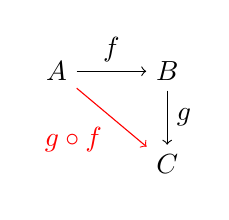
\begin{tikzpicture}[every node/.style={midway}]
\matrix[column sep={4em,between origins},
        row sep={2em}] at (0,0)
{ \node(A)   {$A$}  ; & \node(B) {$B$}; \\
                      & \node(C) {$C$}; \\};
\draw[->] (A) -- (B) node[anchor=south]  {$f$};
\draw[->] (B) -- (C) node[anchor=west]  {$g$};
\draw[->,red] (A) -- (C) node[anchor=north east] {$g\circ f$};
\end{tikzpicture}
\]
We do not really need to draw $g\circ f$ as a separate arrow because the \emph{path} from $A$ to $B$ to $C$ is already implicitly a depiction of $g\circ f$.
So the simpler diagram 
\[
\tikzset{>=stealth}
\begin{tikzpicture}[every node/.style={midway}]
\matrix[column sep={4em,between origins},
        row sep={2em}] at (0,0)
{ \node(A)   {$A$}  ; & \node(B) {$B$}; \\
                      & \node(C) {$C$}; \\};
\draw[->] (A) -- (B) node[anchor=south]  {$f$};
\draw[->] (B) -- (C) node[anchor=west]  {$g$};
\end{tikzpicture}
\]
shows the same information, namely, that $\fromto fAB$ and $\fromto gBC$ are functions and therefore, $g\circ f$ is too.

Now a diagram such as this
\[
\tikzset{>=stealth}
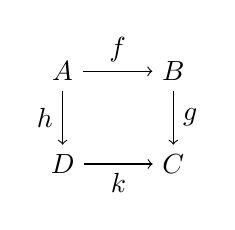
\begin{tikzpicture}[every node/.style={midway}]
\matrix[column sep={4em,between origins},
        row sep={2em}] at (0,0)
{ \node(A)   {$A$}  ; & \node(B) {$B$}; \\
  \node(D)   {$D$}  ; & \node(C) {$C$}; \\};
\draw[->] (A) -- (B) node[anchor=south]  {$f$};
\draw[->] (B) -- (C) node[anchor=west]  {$g$};
\draw[->] (A) -- (D) node[anchor=east] {$h$};
\draw[->] (D) -- (C) node[anchor=north] {$k$};
\end{tikzpicture}
\]
depicts two composite functions $g\circ f$ and $k\circ h$, but $g\circ f$ and $k\circ k$ may not be equal.
We say that the diagram \emph{commutes} or that it is a \emph{commutative diagram} if $g\circ f = k\circ h$.
In other words, saying that a certain diagram commutes \emph{is} an assertion that certain functions are equal.


\begin{exercises}
\begin{enumerate}
\item  For each of the following pairs of functions $\NN\to\NN$, determine whether they are equal and explain why or why not.
  \begin{enumerate}
  \item $f(n) = 2n + 3$ and $g(m) = 2m + 3$
  \item $f(n) = 2^{n+1} - 1$ and $g(n) = \sum_{i=0}^n2^i$
  \item $f(n) =  n^2 + 5n + 6$ and $g(n) = (n+3)(n+2)$
  \item $f(n) = n^4 - 10n^3 + 35n^2 + 50n + 24$ and $g(n) = 24$
  \end{enumerate}
\item Let $\RR$ denote the set of all real numbers. Let $f(x) = \tan(x)$.
Explain why this does \emph{not} define a function from $\RR$ to $\RR$.
\item Suppose the following functions exist: $\fromto fAB$, $\fromto gBC$, $\fromto aAD$, $\fromto bCD$. 
  Draw a commutative diagram asserting that $b\circ g\circ f = a$.
\item Suppose the following functions exist: $\fromto fCA$, $\fromto gCB$, $\fromto hCP$, $\fromto pPA$ and $\fromto qPB$.
 Draw a commutative diagram asserting that $f=p\circ h$ and $g=q\circ h$.
\end{enumerate}
\end{exercises}

\chapter{Basic Building Blocks}

\begin{goals}
	\noindent\textbf{Lecture}
	\begin{itemize}
	\item Characterize and define
		 \begin{itemize}
			 \item Pointer and constant functions
			\item Solution sets
			\item Characteristic functions
			%		 	\item The set of natural numbers
			\item Products of sets
			\item Exponents of sets
		 \end{itemize}
	\item Introduce the idea of a \emph{universal} construction.
	\end{itemize}

	\noindent\textbf{Study}
	\begin{itemize}
	\item Be able to calculate membership in various constructed sets 
	\item Learn to use universal constructions to define functions. 
	\end{itemize}
\end{goals}

So far, we have been able to think mainly about finite sets and a few informally defined functions on, say, the real numbers or the natural numbers.
To fill out our understanding of sets, we need to be able to build sets for specific purposes.

Two finite sets will play particularly important roles.
The first, which we denote by $\One$, is  set with one element; the second, which we denote by $\Two$, is a set with two elements.
It does not matter at all \emph{what} elements are in these because, as we will soon see, any two sets of the same size are interchangeable.
What `interchangeable' means is discussed later.
What `same size' means is obvious for finite sets, but not at all apparent for infinite ones.
We discuss the general situation later as well.

For the time being, we merely need to agree on a fixed set with one element and a fixed set with two elements.
The particular choices I make here will be clearer as we put them to use.

\begin{defn}
	Let $\bullet$, $\bot$ and $\top$ be fixed symbols. Then define
	\begin{align*}
		\One &= \{\bullet\}\\
		\Two &= \{\bot,\top\}
	\end{align*} 
	The single element of $\One$ is intended to look like a generic point in an internal diagram.
	The element $\top$ is meant to remind you of the letter `T' (short for `True') and $\bot$ is meant to be the opposite of $\top$ (that is, 'False').
\end{defn}


\section{Elements, Pointers and Constant Functions}

Suppose we are told that $\fromto p\One A$ is a function.
Since $\bullet\in\One$, this function determines an element of $A$, namely $p(\bullet)$.
A picture of the situation might be this:
\[
  \begin{tikzpicture}[
    >=stealth,
    bullet/.style={
      fill=black,
      circle,
      minimum width=1pt,
      inner sep=1pt
    },
    projection/.style={
      ->,
      thick,
      shorten <=2pt,
      shorten >=2pt
    },
    every fit/.style={
      ellipse,
      draw,
      inner sep=0pt
    }
  ]
    \node[bullet] (p) at (0,2.5) {};

    \foreach \x/\y/\l in {4.1/1/4,3.2/2/3,4.3/3/2,4/4/1}
      \node[bullet,label=right:$\l$] (a\y) at (\x,\y) {};

    \node[draw,fit=(p),minimum width=1cm, minimum height=1cm] {} ;
    \node[draw,fit=(a1) (a2) (a3) (a4),minimum width=2cm] {} ;

    \draw[projection] (p) -- (a3);
  \end{tikzpicture}
\]
Since $\One$ has only a single element, it can ``point'' only to a single element of $A$.
So we might refer to a function $\One\to A$ as a \emph{pointer} into $A$.
Each pointer determines an element of $A$. 
And conversely, it should be possible to point to any element of $A$. 
This leads to our first axiom guaranteeing that certain functions exist.

\begin{principle}\label{ax:pointers}
	For any set $A$, and any $a\in A$, there is a pointer $\fromto {\hat a}\One A$ so that $\hat{a}(\bullet)=a$.
\end{principle}

In effect, this principle claims that elements of a set $A$ and functions $\One\to A$ are interchangible: from $a\in A$ we get $\fromto {\hat{a}}\One A$; from $\fromto p\One A$.
we get $p(\bullet)$. 

This principle also justifies the drawing of internal diagrams for pointers because it means that any such diagram does depict an actual function. 
Other principles that we will discuss later justify our use of internal diagrams for all finite sets.

We can specify $\hat{a}$ by the rule $x\mapsto a$.
That is, since $\bullet$ is an element of $\One$, $\hat{a}(\bullet)=a$.
And since $\bullet$ is the only element of $\One$, $\hat{a}{x}=a$ is true for \emph{every} element of $\One$.

Suppose $\fromto fA\One$ and $\fromto gA\One$ are functions, that is, their \emph{codomain} is $\One$ instead their \emph{domain}. 
Then $f(a)=g(a)$ is true for every $a\in A$ because $\bullet$ is the only possible value for $f(a)$ and $g(a)$. 
So $f=g$ by the Principle of Function Extensionality.
In other words, there is at most one function from $A$ to $\One$.
But the rule $x\mapsto \bullet$ is as simple a rule as one can imagine. 
This leads to another axiom.

\begin{defn}\label{def:terminal}
	A set $T$ is \emph{terminal} if it is the case that for any set $A$ there is exactly one function from $A$ to $T$.
\end{defn}

\begin{principle}
	The set $\One$ is a terminal set. 
	We denote the unique function from $A$ to $\One$ by $\fromto {\Diamond_A}{A}\One$.
	
	The rule defining $\Diamond_A$ must be
	\[x\mapsto\bullet\]
	because no other rule is possible. 
\end{principle}

Using $\Diamond_A$ and $\hat{b}$ for an element $b\in B$, we can now define constant functions. 
That is $\hat{b}\circ\Diamond_A$ is a function from $A$ to $B$ defined by 
\[(\hat{b}\circ\Diamond_A)(x) = \hat{b}(\Diamond_A(x))= \hat{b}(\bullet) = b.\] 
In short, this is the function sending any element of $A$ to the constant result $b$. 

\begin{exercises}
	\begin{enumerate}
		\item Show that for any pointer $\fromto p\One A$, it is the case that $\widehat{p(\bullet)}=p$.
		\item Show that any set with exactly one element is a terminal set.
		\item Suppose that $\fromto fAB$ is a function. Show that for every $a\in A$, $\widehat{f(a)} = f\circ \hat{a}$.
	\end{enumerate}
\end{exercises}

\section{The Empty Set}

For trivial reasons, there is at most one function from $\emptyset$ to $A$,
for any set $A$. That is,  if $\fromto {f,g}\emptyset A$ are functions, then
for each $x\in\emptyset$, $f(x)=g(x)$ because there are none. Hence by Principle \ref{ax:FunctionExtensionality}, $f=g$. The empty ``rule'' that tells us nothing does actually specify a function from $\emptyset$ to $A$. So $\emptyset$ 
is the \emph{initial} set, i.e., for any set $A$, there is exactly one function from $\emptyset$ to $A$.

\begin{defn}
	An \emph{initial set} is a set $I$ so that for any set $A$, there is exactly one function from $I$ to $A$.
\end{defn}

\begin{principle}
	The emptyset $\emptyset$ is an initial set.
\end{principle}

Notice that a function $A\to\emptyset$ is impossible unless $A$ is also empty.
So it follows that $\emptyset$ is the only initial set. 

\begin{exercises}
	\begin{enumerate}
		\item How many functions are there from $\emptyset$ to $\{a,b,c,d\}$
		\item How many functions are there from $\{a,b,c,d\}$ to $emptyset$.
	\end{enumerate}
\end{exercises}


\section{Solution Sets, Subsets, Characteristic Functions}

Suppose we are given two functions that are ``parallel'': $\fromto fAB$ and $\fromto gAB$.
Then for some value $a\in A$, it might be the case that $f(a)=g(a)$.
We may call such a value a \emph{particular solution to the equation $f(x)=g(x)$}. 
It might be the case that there are no particular solutions.
For example, there are no natural numbers $n$ such that $n+1 = n$. 
On the other hand, there might be many particular solutions. 
For example, let $f(x)=x^3$ and let $g(x)= 6x^2 - 11x + 6$ both as functions on the natural numbers.
Then it is easy to check that $1$, $2$ and $3$ solve the equation.
In fact, these three are the only particular solutions.
We generalize as follows.

\begin{defn}\label{def:equalizer} 
	For two functions $A\doublerightarrow{f}{g} B$, a \emph{solution} is a function $\fromto sCA$ so that 
	\[f\circ s = g\circ s.\]
	Thus for example, if $a\in A$ is a particular solution then the pointer $\hat a$ is a solution. 

	For functions $\fromto fAB$ and $\fromto gAB$, an \emph{equalizer} is solution $\fromto eEA$ so that for any solution $\fromto sCA$, there is exactly one function $\fromto hCE$ so that \[e\circ h = k.\]
\end{defn}

\begin{principle}
	For functions $A\doublerightarrow{f}{g} B$, the collection of all particular solutions to the equation $f(x)=g(x)$ form a set, denoted by $\{x\in A\st f(x) = g(x)\}$. 	
	The function $\fromto i{\{x\in A\st f(x)=g(x)\}}A$ given by the rule $x\mapsto x$ (called an \emph{inclusion map}) is an equalizer for $f$ and $g$.
	
	If $\fromto sCA$ is a solution of  $f(x)=g(x)$, that is, $f\circ s = g\circ s$,
	then the function $\fromto {\check s}C{\{x\in A\st f(x)=g(x)\}}$ given by the rule $x\mapsto s(x)$
	is the unique function for which $s = i\circ \check s$. 
\end{principle}

This axiom tells us three main things.
First, we can form a subset of $A$ by specifying an equation $f(x)=g(x)$ for any two functions $A\doublerightarrow{f}{g}B$, and picking out the particular solutions.
Second, a subset formed in this way ``embeds'' in the given set $A$ by its inclusion map $i$.
Third, for any solution $s$, the function into the set of particular solutions is defined by the same rule as $s$.

Suppose $c\in C$ and $\fromto fAC$ is a function, then we can form the equalizer of $f$ and the constant function $\hat{c}\circ\Diamond_A$.
This is more easily written we $\{x\in A\st f(x)=c\}$.
Since it common to pick out sets like this, special notation is in order.

\begin{defn}\label{def:inverse-image}
	For a function $\fromto fAC$, and a value $c\in C$, 
	\[f^{-1}(c) = \{x\in A\st f(x)=c\}.\] 
	In this case, $f^{-1}(c)$ is called the \emph{inverse image of $c$ with respect to $f$}.
\end{defn}

Evidently, in Definition \ref{def:inverse-image}, the set $f^{-1}(c)$ is a subset of $A$.
It would be good to know that any subset of $A$ can be described as an inverse image.
This is where the set $\Two$ plays a role.

\begin{defn}\label{def:subset-classifier}
	A \emph{subset classifier} is a set $S$ with a distinguished element $t\in S$ so that for any set $A$ and any subset $B\subseteq A$, there is exactly one function $\fromto kAT$ for which $B = k^{-1}(t)$.
	That is, $B$ is uniquely defined as the inverse image of $t$ with respect to a function into $T$.
\end{defn}

\begin{principle}\label{ax:subset-char}
	The set $\Two$ with the distinguished element $\top$ is a subset classifier.
	For subset $B\subseteq A$, the function corresponding to $B$, called the \emph{characteristic function of $B$}, is denoted by $\kappa_B$.
	In other words, $\kappa_B$ is the unique function for which $B = \kappa_B^{-1}(\top)$.

	For $B\subseteq A$, the characteristic function is defined by the rule
	\[
	x \mapsto
		\begin{cases}
			\top &\text{ if } x\in B\\
			\bot &\text{ otherwise}
		\end{cases}
	\]
\end{principle}

Just as Principle \ref{ax:pointers} asserts that elements of $A$ and functions $\One\to A$ are interchangeable, Principle \ref{ax:subset-char} asserts that the subsets of $A$ and the functions $A\to\Two$ are interchangeable.

\begin{exercises}
	\begin{enumerate}
	\item Draw a depiction of $A=\{a,b,c,d,e,f,g\}$ and its subset $B=\{a,c,e,g\}$ in the same internal diagram. Now depict the characteristic map for $B$ as a subset of $A$.
	
	\item Define two functions $\NN\doublerightarrow{f}{g}\NN$ so that the set of particular solutions fo $f(x)=g(x)$ is $\{1,5\}$. 
	
	\item Consider the functions $\fromto f\RR\RR$ defined by $f(x) = \sin(x) + \cos(x)$, and $\fromto s\NN\RR$ defined by $s(n) = 2\pi n^2$. 
	Is $s$ a solution for the equation $f(x) = -1$? 
	What is the set of all particular solutions?
	\end{enumerate}
		
\end{exercises}

\section{Product Sets and Functions of Two Arguments}

We should be able to deal with functions of more than one argument, such as a function $f(x,y) = x+y$.
To account for these, we take our cue from Descartes.

Descartes studied the geometric plane in terms of a coordinate system consisting of the so-called $x$-axis and $y$-axis (what we call cartesian coordinates in his honor).
Once we have decided where to place the axes (as long as they do not run in parallel), a pair such as $(2,3)$ determines a point on the plane, and any point $p$ in the plane determines a pair.
So Descartes realized that we might as well just say that the plane actually \emph{is} the collection of all pairs of real numbers.
What makes this work is that points in the plane \emph{project} onto the two axes in a universal way.
Products of sets generalize this idea.

\begin{defn}
For sets $A$ and $B$, a \emph{table} consists of two functions $A\stackrel{f}{\longleftarrow} C\stackrel{g}{\longrightarrow}B$.
Note that the two functions have the same domain. We may call the two functions \emph{legs} of the table.

For sets $A$ and $B$, a \emph{product of $A$ and $B$} is a table $A\stackrel{p}{\longleftarrow} P\stackrel{q}{\longrightarrow}B$ so that for any table $A\stackrel{f}{\longleftarrow} C\stackrel{g}{\longrightarrow}B$ there is exactly one function $\fromto hCP$ for which $f = p\circ h$ and $g= q\circ h$. 
For a product, the legs $p$ and $q$ are called the \emph{projections}.
\end{defn}

\begin{principle}\label{ax:products}
	For sets $A$ and $B$, the collection of all pairs $(a,b)$ where $a\in A$ and $b\in B$ is a set, denoted by $A\times B$. 
	The functions $\fromto {\pi_0}{A\times B}A$ and $\fromto {\pi_1}{A\times B}B$ defined by $\pi_0(a,b)=a$
	and $\pi_1(a,b)=b$ are projections. For $\fromto fCA$ and $\fromto gCB$, the unique function required by
	the product may be denoted by $\langle f,g\rangle$.

	For $\fromto fCA$ and $\fromto gCB$, the function $\fromto {\langle f,g\rangle}C{A\times B}$ is defined by the rule $\langle f,g\rangle(x)=(f(x),g(x))$.
\end{principle}

Suppose we are given two unrelated functions $\fromto fAB$ and $\fromto gCD$. 
We can now form a single function from $A\times C$ to $B\times D$ by combining $f$ and $g$ ``independently''. 
That is, define $f\times g = \langle f\circ \pi_0,g\circ \pi_1\rangle$.
Calculating concretely in terms of elements $(f\times g)(x,y) = (f(x),g(y))$. 
So $f\times g$ acts on a pair $(x,y)$ by applying $f$ to $x$ and unrelatedly applying $g$ to $y$. 

\begin{exercises}
	\begin{enumerate}
		\item For the sets $A = \{a,b,c\}$ and $B = \{1,2,3,4\}$, calculate $A\times B$ and $B\times A$
		\item What is $\emptyset \times A$? 
		\item Calculate $\{4,a,0\}\times \Two$.
		\item Describe in plain English what are the elements of $\NN\times \NN$.
		\item Suppose $A$ is a finite set with $m$ elements and $B$ is a finite set with $n$ elements.
		How many elements are in $A\times B$?
		Describe in plain English why it makes sense to refer to $A\times B$ as a ``product.''
	\end{enumerate}
\end{exercises}

\section{Function Sets}

A function from $A$ to $B$ might depend on a parameter from $C$. 
For example, the function $\fromto f\RR\RR$ defined by the rule $f(x) = \sin(x + c)$ depends on the constant $c$.
There is a related function $\fromto g{\RR\times \RR}\RR$ defined by $g(c,x) = \sin(x+c)$.
Evidently, $g$ describes the same behavior as $f$, but it makes the parameter explicit.
This leads to the following definition.

\begin{defn}
	For sets $A$ and $B$, a \emph{parametric function from $A$ to $B$} is a function $\fromto g{C\times A}B$ for some set $C$.
	The set $C$ may be called the \emph{set of parameters}.
	
	Suppose $\fromto f{D\times A}B$ is a parametric function with parameter set $D$ and $\fromto kCD$ is a function.
	Then we can form another parametric function with parameters in $C$ by composition: $f\circ (k\times \id_A)$.
	We may refer to $k$ as a \emph{change of parameters} function because $k$ transforms the parametric function with parameters in $D$ into a parametric function with parameters in $C$. 
	Specifically, $f\circ(k\times \id_A)$ is given by the rule $(c,a)\mapsto f(k(c),a)$. 
	
	An \emph{evaluation map} for $A$ and $B$ is a parametric function $\fromto a{F\times A}B$, so that for any 
	parametric function $\fromto g{C\times A}B$ there is exactly one change of parameters $\fromto hCF$ so that
	$g = a\circ (h\times \id_A)$. In that case, $F$ is called a \emph{function set} or an \emph{exponential}.
\end{defn}

\begin{principle}
	For sets $A$ and $B$, the collection of all functions from $A$ to $B$, denoted by $B^A$, is a set.
	Moreover, there is an evaluation map $\fromto \appl{B^A\times A}B$ defined by the rule $(f,x) \mapsto f(x)$.
	The unique change of parameters function corresponding to $\fromto f{C\times A}B$ does not have a completely standard name.
	Some mathematicians honor the twentieth century logician names Haskell Curry by referring to this as `currying'.
	For these lectures, we follow that tradition and write $\curry[f]$ for the unique function satisfying $f = \appl\circ (\curry[f] \times \id_A)$.
	
	Calculating how $\fromto {\curry[f]}C{B^A}$ must behave, we see that $\curry[f](c)$ is the function from $A$ to $B$ given by the rule $x\mapsto f(c,x)$.
	So for any $c\in C$ and $a\in A$, $\curry[f](c)(a) = f(c,a)$. 
\end{principle}

\subsection*{$\lambda$ Notation}

When we describe a function by  rule like $x\mapsto x^2$, it is usually convenient to give the function a name.
So we might write $f(x) = x^2$.
But sometimes, it is also convenient to have a notation for a function without giving it an explicit name. 
The logician Alonzo Church \cite{church} proposed a simple notation to describe functions. 
He wrote things like $\lambda x.x^2$ to describe the function that squares its input. 
The Greek letter $\lambda$ is used merely as a marker to introduce a function. 
It does not mean anything special. 
We could make the $\lambda$ notation formal, but for our purposes we do not need that.

\begin{example}
	Suppose $\fromto fAB$ and $\fromto gBC$. Then $g\circ f$ is the function
	$\lambda x.g(f(x))$.  So $f\in B^A$ and $g\in C^B$ determine $g\circ f\in C^A$.
	Thus $\circ$ can be regarded (locally) as a function $B^A\times C^B\to C^A$.
	It is defined by $\lambda(f,g).\lambda x.g(f(x))$.
\end{example}
 

\begin{exercises}
	\begin{enumerate}
		\item  For set $A= \{1,2,3\}$ and $B = \{a,b\}$ 
			\begin{enumerate}
				\item draw internal diagrams corresponding to each element of $B^A$ (there are eight of them);
				\item draw internal diagrams corresponding to each element of $A^B$ (there are nine of them).
			\end{enumerate}
		\item Consider the function $\fromto f{\NN\to\NN}\NN$ defined by
		      $f(m,n) = m^n$. What function is $\curry[f](3)$? Use $\lambda$ notation to describe it.
	\end{enumerate}	
\end{exercises}

\section{Universal Constructions}

Consider the product $A\times B$ again.
It possesses functions 
$A\stackrel{\pi_0}{\longleftarrow}A\times B\stackrel{\pi_1}{\longrightarrow}B$. For any other similar arrangement
$A\stackrel{f}{\longleftarrow}C\stackrel{g}{\longrightarrow}B$, there is a unique function $C\stackrel{\langle f,g\rangle}{\longrightarrow}{A\times B}$ making the diagram
\[
\tikzset{>=stealth}
\begin{tikzpicture}[every node/.style={midway}]
\matrix[column sep={4em,between origins},
row sep={2em}] at (0,0) {};
%{ & \node(T)   {$T$}  ; & \\
%	\node(A)   {$A$}  ; & \node(P) {$P$}; & \node(B) {$B$} \\};
%\draw[->] (T) -- (A) node[anchor=north]  {$f$};
%\draw[->] (T) -- (B) node[anchor=north]  {$g$};
%\draw[->] (T) -- (P) node[anchor=east] {$\lange f,g \rangle$};
%\draw[->] (P) -- (A) node[anchor=south] {$\pi_0$};
%\draw[->] (P) -- (B) node[anchor=south] {$\pi_1$};
\end{tikzpicture}
\]
commute.

An equalizer ($\{x\in A\st f(x)=g(x)\}$), a terminal object ($\One$) and an exponential ($B^A$) are also characterized by some special functions so that any similarly arranged functions determine a unique function making a suitable diagram commute. Go back and reread the definitions of equalizers, terminal objects, products and exponentials to see that they all have this family resemblance. They are called \emph{universal constructions}. So the inclusion $\{x\in A\st f(x)=g(x)\}\to A$ is universal for solving the equation $f=g$; $A\stackrel{\pi_0}{\longleftarrow}A\times B\stackrel{\pi_1}{\longrightarrow}B$ is universal for mapping into $A$ and $B$;
$B^A\times A\stackrel{\appl}B$ is the universal parametric function from $A$ to $B$. The principes of this lecture spell out that there are sets and functions 
with the desired universal properties.

\begin{exercises}
	\begin{enumerate}
		\item Explain how $\One\stackrel{\hat{\top}}{\longrightarrow}\Two$ is universal. [There is not a set answer to this. I want you to think about how $\Two$ fits into a bigger picture.]
	\end{enumerate}
\end{exercises}



\chapter{Powersets and Internal Logic}

The exponential $\Two^A$ for any set $A$ is the set of all characteristic maps on $A$.
So the elements of $\Two^A$ correspond to subsets of $A$, and vice versa.
It makes sense also to suppose that the actual collection of subsets of a set $A$ form a set.
This behaves exactly like $\Two^A$, but concretely, it consists of sets rather than characteristic functions.

\begin{principle}\label{ax:powerset}
	For any set $A$, the collection of subsets of $A$ is a set, denoted by $\powerset(A)$, and called the \emph{power set of $A$}. Moreover, there is a function $\fromto {\ni_A}{\powerset(A)\times A}\Two$ defined by 
	\[\ni_A(B,x) = \begin{cases}
		\top, &\text{ if } x\in B\\
		\bot &\text{otherwise}
	\end{cases}
	\]
	The function $\ni_A$ is an evaluation map, meaning that 
	for any function $\fromto f{C\times A}\Two$, there is a unique function $\fromto {\overline{f}}C{\powerset(A)}$ for which $f = \ni_A\circ (\overline{f} \times \id_A)$. The function $\overline f$ 
	is given by the rule $c\mapsto \{x\in A\st f(c,x)=\top\}$.
\end{principle}

For a function $\fromto fAB$, $\ni_B\circ (\id_{\powerset(B)}\times f)$ is a function from $\powerset(B)\times A$ to $\Two$. So there is a unique function
from $\powerset(B)$ to $\powerset(A)$ determined by it. 

\begin{defn}
	For $\fromto fAB$, let $\fromto {f^{-1}}{\powerset(B)}{\powerset(A)}$ denote
	the unique function for which $\ni_B\circ (\id_{\powerset(B)}\times f) = \ni_A\circ(f^{-1}\times \id_A)$. In simpler terms, $f^{-1}$ satsifies
\[x\in f^{-1}(Y) \text{if and only if } f(x)\in Y\]
for every $Y\subseteq B$.  So $f^{-1}$ is given by the rule $Y\mapsto \{x\in A\st f(x)\in Y\}$
\end{defn}

This notation does not clash much with our usage of $f^{-1}(b)$ because 
$f^{-1}(b)$ (from the earlier usage) is the same as $f^{-1}(\{b\})$.

\section{Specifying Subsets}

We have introduced the notation $\{x\in A\st f(x)=g(x)\}$ to specify the subset of $A$ consisting of the particular solutions to the equation $f(x)=g(x)$. 
We have also slightly extended this for inverse images of elements: $\{x\in A \st f(x)=b\}$, and inverse images of subsets: $\{x\in A\st f(x)\in Y\}$. 
Life would be easier if we had a more general system for specifying subsets, whereby we could write things like $\{n\in \NN \st \text{$n$ is prime}\}$, or $\{f\in \RR^\RR\st \text{$f$ is differentiable}\}$, or $\{(x,y)\in \RR\times \RR\st |x-y| < \epsilon\}$. 

As it happens, all of these examples are honest specifications of subsets. 
The fact that two of them use English is not a problem, as long as what we write is unambiguous. 
In contrast, $\{x\in \RR\st \text{$x$ is messy}\}$ is probably not a good specification, unless we make the meaning of ``messy'' precise. 
So in practical situations, it is harmless to write clear unambiguous plain language as part of a specification. 
Nevertheless, it is also helpful to have in mind some formal aspects of this notation, and to put some effort into sorting out when an expression of the form
$\{x\in U\st \ldots x \ldots\}$ makes sense.

First, we need to understand what is means for a variable to \emph{appear free} in an expression.
In $\{x\in A \st f(x)=g(x)\}$ the variable \emph{appears bound}.
This means, roughly, that the meaning of the expression does not depend on a value for $x$, so we are not ``free'' to interpret $x$.
In contrast, $f$ and $g$ appear free in the same expression because the meaning of the expression depends on the meanings of $f$ and $g$.
We are ``free'' to choose what they mean.
Similarly, in the English phrase, ``$m + n = n + m$ for all natural numbers $m$ and $n$'' the variables $m$ and $n$ are bound.
But in the phrase ``$m+k = n$ for some $k$'' the variables $m$ and $n$ are free and the variable $k$ is bound.
An important feature of bound variables is that we may rename them without changing the meaning, so long as we do so systematically.
For example, ``$m+j=n$'' for some $j$'' means exactly the same as ``$m+k=n''$ for some $k$''.
But we can't just swap $m$ for some other variable without changing the meaning. 

In the following, we write $P(x,y,z)$ for an expression in which $x$, $y$ and $z$ may appear, but are not required. 
We can allow expressions in a mix of English and mathematical notation, so long as the meanings are clear.

\begin{vocabulary}
	In the following, let $X$ and $W$ be sets. Let $P(x)$, $Q(x)$, $R(w,x)$ be expressions and $A,B\subseteq X$, $C\subseteq X\times X$ so that
	\begin{itemize}
		\item $A = \{x\in X\st P(x)\}$,
		\item $B = \{x\in X\st Q(x)\}$, and
		\item $C = \{(w,x)\in W\times X\st R(w,x)\}$.
	\end{itemize}
Then the following sets are definable. 
\begin{itemize}
\item $W\times A = \{(w,x)\in W\times X\st P(x)\}$. In fact, this is the same 
as $\pi_1^{-1}(A)$.  

\item $A\cap B = \{x\in X\st \text{$P(x)$ and $Q(x)$}\}$. We may abbreviate ``$P(x)$ and $Q(x)$'' by writing ``$P(x)\wedge Q(x)$''. 

\item $A\Rightarrow B = \{x\in X\st \text{$P(x)$ implies $Q(x)$}\}$. We may abbreviate ``$P(x)$ implies $Q(x)$'' by writing ``$P(x)\to Q(x)$''.

\item $A\cup B = \{x\in X\st \text{$P(x)$ or $Q(x)$}\}$. We may abbreviate ``$P(x)$ or $Q(x)$'' by writing ``$P(x)\vee Q(x)$''.
	
\item $\emptyset = \{x\in X\st \text{false} \}$. This defines $\emptyset$ as a subset of $A$. We may abbreviate ``false'' by writing $\textsf{F}$.
	
\item $X = \{x\in X\st \text{true}\}$ defines $X$ as a subset of $X$. We may abbreviate ``true'' by writing $\textsf{T}$.
	
\item $\{x\in X \st \text{for some $w\in W$, $R(w,x)$}\}$ defines a subset of $X$. We may abbreviate ``for some $w\in W$, $R(w,x)$'' by writing ``$\exists w\in W, P(w,x)$''.
	
\item $\{x\in X \st \text{for every $w\in W$, $R(w,x)$}\}$ defines a subset of $X$.  We may abbreviate ``for every $x\in W$, $R(w,x)$'' by writing ``$\forall w\in W, R(w,x)$''.

\item $A^* = \{x\in X\st \text{it is not the case that $P(x)$}\}$.  We may abbreviate ``it is the case that $P(x)$'' by writing ``$\neg P(x)$''.
\end{itemize}
\end{vocabulary}

All of these can defined as equalizers $\{x\in X\st k(x)=\top\}$ for suitable choices of $k$, but the exercise of finding the suitable choices is not likely to be illuminating for now. 
The point here is simply that, together with equalizers and inverse images, these constructions provide a rich system for describing subsets of given sets.
Also note that $A^*$ is the same thing as $A\Rightarrow\emptyset$ because $x\in A^*$ means that $x\in X$ and $x\notin A$.
But $x\in A\Rightarrow \emptyset$ means $x\in AX$ and \emph{if $x\in A$, then $x\in\emptyset$}.
The only elements of $X$ that can satisfy the latter condition are those that are not in $A$.

\section{The structure of Powersets}
  
For any set $U$, the powerset $\powerset(U)$ has useful structure.
It is a \emph{partially ordered set} with respect to $\subseteq$.
This means that $\subseteq$ satisfies three conditions:
\begin{description}
	\item[Reflexivity] $A\subseteq A$ holds for any $A\in \powerset(U)$;
	\item[Transitivity] If $A\subseteq B$ and $B\subseteq C$, then $A\subseteq C$ for any $A,B,C\in\powerset(U)$;
	\item[Anti-symmetry] If $A\subseteq B$ and $B\subseteq A$, then $A=B$. 
\end{description}

More specifically, $\powerset(U)$ is known as a \emph{complete atomic Boolean algebra}. In an important sense, this is \emph{the} structure of a powerset. So we
should take some time to understand it. First, let us consider how the basic
constructions of the previous section behave.

\begin{lemma}
	For a set $U$ and subsets $A$, $B$ and $C$,
\[\text{$C\subseteq A\cap B$ if and only if $C\subseteq A$ and $C\subseteq B$.}\]
	
	\begin{proof}
		Suppose $C\subseteq A\cap B$.
		Since $x\in A\cap B$ implies, by definition,
		that $x\in A$ and $x\in B$, obviously $C\subseteq A$ and $C\subseteq B$.
		
		Suppose $C\subseteq A$ and $C\subseteq AB$, and consider some $x\in C$.
		Then $x\in A$ and $x\in B$, so by definition $x\in A\cap B$.
	\end{proof}
\end{lemma}

\begin{lemma}
	For a set $U$ and subsets $A$, $B$ and $C$,
	\[\text{$A\cup B\subseteq C$ if and only if $A\subseteq C$ and $B\subseteq C$.}\]
	
	\begin{proof}
		Exercise.
	\end{proof}
\end{lemma}

From these, it is easy to see that $\cap$ and $\cup$ are commutative, associative
and idempotent. That is,

$A\cap B = B\cap A$
$A\cap (B\cap C) = (A\cap B)\cap C$
$A\cap A = A$

A binary operation that satisfies these three laws is called a \emph{semilattice} operation. But actually $\cap$ and $\cup$ interact by another law.
$A\cap (B\cup A) = (A\cap B)\cup A$

Any structure with two operations that satisfy all of these laws is called a \emph{lattice}. So $\powerset(X)$ with the operations $\cap$ and $\cup$ is a lattice. If the two operations have identities $A\cap X = A$ and $a\cup \emptyset = A$, then it is a \emph{bounded lattice}. 

So in fact, $\powerset(X)$ with $\cap$, $\cup$, $X$ and $\emptyset$ forms a bounded lattice. Next, we consider how $\Rightarrow$ provides additional information.

\begin{lemma}
	For set $X$ and subsets $A$, $B$ and $C$,
	\[\text{$A\cap B\subseteq C$ if and only if $A\subseteq B\Rightarrow C$}\]
	
	\begin{proof}
		Suppose $A\cap B\subseteq C$. Consider $x\in A$. 
		For such an $x$, it i true that $x\in B$ implies $x\in C$.
		So $x\in B\Rightarrow C$.
		
		Suppose $A\subseteq B\Rightarrow C$.
		Consider $x\in A\cap B$. 
		Then $x\in A$. So $x\in B\Rightarrow C$.
		But also $x\in B$. So $x\in C$. 		
	\end{proof}
\end{lemma}

This law, sometimes called the Law of Residuation, specifies exactly how $\cap$ an $\Rightarrow$ interact. A bounded lattice with an operation that satisies the Law of Residuation is called a \emph{Heyting algebra}. So we have not shown that $\powerset(X)$ is a Heyting algebra. A useful fact about Heyting algebras is that, even though residuation does not explicitly mention $\cup$, it implies that law of distribution.

\begin{lemma}
	For set $X$ and subsets $A$, $B$, and $C$,
	\[A\cap (B\cup C) = (A\cap B) \cup (A\cap C)\]
	
	\begin{proof}
		In any lattice $(A\cap B)\cup (A\cap C)\subseteq A\cap (B\cup C)$. [Prove this as an exercise.]
		So the equality only requires we prove the other inclusion.
		
		By the Law of Residuation, $A\cap (B\cup C)\subseteq (A\cap B)\cup (A\cap C)$ holds if and only if $B\cup C\subseteq A\Rightarrow (A\cap B)\cup (A\cap C)$ holds. But by Law of Union, the latter holds if and only if both $B\subseteq A\Rightarrow ((A\cap B)\cup (A\cap C))$ and $C\subseteq A\Rightarrow ((A\cap B)\cup (A\cap C))$ hold. And finally, by the Law of Residuation again, $B\subseteq A\Rightarrow ((A\cap B)\cup (A\cap C))$ holds if and only if $A\cap B\subseteq (A\cap B)\cup (A\cap C)$ holds, and likewise for $C$. But $A\cap B$ is indeed contained in $(A\cap B)\cup (A\cap C)$ and similarly $A\cap C$ is indeed contained in $(A\cap B)\cup (A\cap C)$. 
	\end{proof}
\end{lemma}

Notice that the proof does not explicitly mention elements of $X$. It only uses the algebraic properties of $\cap$, $\cup$ and $\Rightarrow$. So we have actually proved that every Heyting algebra satisfies the Law of Distribution.

\begin{lemma}
	For set $X$ and subset $A\subseteq X$, $A^{**} = A$.
	
	\begin{proof}
		Exercise.
	\end{proof}
\end{lemma}

A Heyting algebra satisfying this additional law is called a Boolean algebra (historically, this is backwards. Boolean algebras were named before Heyting algebras). So $\powerset(X)$ is a Boolean algebra.

\begin{lemma}
	For any function $\fromto fXY$, the function $\fromto {f^{-1}}{\powerset(Y)}{\powerset(X)}$ satisfies
	\begin{itemize}
		\item $f^{-1}(\emptyset) = \emptyset$
		\item $f^{-1}(A\cup B) = f^{-1}(A)\cup f^{-1}(B)$
		\item $f^{-1}(Y) = X$
		\item $f^{-1}(A\cap B) = f^{-1}(A) \cap f^{-1}(B)$
		\item $f^{-1}(A^*) = f^{-1}(A)^*$
	\end{itemize}
\end{lemma}

So not only is $\powerset(X)$ always a Boolean algebra, but $f^{-1}$ is a function that \emph{preserves} the relevant operations that give $\powerset(X)$ that structure.

An element $x$ of a Boolean algebra is \emph{atomic} if whenever $x = y\vee z$,
either $y=x$ or $z=x$. In $\powerset(X)$, the atoms are singleton subsets $\{x\}$
for $x\in X$. In $\powerset(X)$, there are a lot of atoms. Specifically, 
every $A\in\powerset(X)$ is either $\emptyset$ or has at least one atom $\{x\}\subseteq A$. It is possible to have a Boolean algebra with no atoms, but this is a property that all powersets have.

Summarizing so far $\powerset(X)$ is an atomic Boolean algebra, and $f^{-1}$ preserves Boolean structure. Since $f^{-1}(\{x\})$ is not necessarily a singleton,
$f^{-1}$ does not generally preserve atoms.

Finally, we need to understand completeness.

\begin{lemma}
	For sets $W$ and $X$, expression $P(w,x)$ defining $\{(w,x)\in W\times X\st P(w,x)\}$ and $A\subseteq X$,
	\[\text{$\{x\in X\st \exists w\in W.P(w,x)\} \subseteq A$ if and only if $\{(w,x)\in W\times X\st P(w,x)\} \subseteq \pi_1^{-1}(A)$.}\] 
	 
	\begin{proof}
		Suppose $\{x\in X\st \exists w\in W.P(w,x)\}\subseteq A$.
		Consider $(w,x)\in W\times X$ for which $P(w,x)$.
		Then $x\in A$. So $(w,x)\in \pi_1^{-1}(A)$. 
		
		For the reserve inclusion, suppose $\{(w,x)\in W\times X\st P(x,y)\}\subseteq \pi_1^{-1}(A)$.
		Consider $x\in X$ for which $P(w,x)$ holds for some $w\in W$.
		Then $(w,x)\in \pi^{-1}(A)$.
		So $x\in A$.
	\end{proof}
\end{lemma}

\begin{lemma}
		For sets $W$ and $X$, expression $P(w,x)$ defining $\{(w,x)\in W\times X\st P(w,x)\}$ and subset $A\subseteq X$,
		\[\text{$A\subseteq \{x\in X\st \forall w\in W.P(w,x)\}$ if and only if 
		$\pi_1^{-1}(A)\subseteq \{(w,x)\in W\times X\st P(w,x)\}$.}\]
		
		\begin{proof}
			Exercise.
		\end{proof} 	
\end{lemma}

First, for completeness we need the following definition:
\begin{defn}
	Let $\fromto aIA$ be a function. Writing $a_i$,
	instead of $a(i)$, then we refer to $a$ as an \emph{(indexed) family of elements of $A$}, and write it as $\{a_i\}_{i\in I}$. This notation is just a way to denote a function that emphasizes its role as a way to pick out elements of $A$.
	
	If $(P,\leq)$ is a partially ordered set and $\{a_i\}_{i\in I}$ is an indexed family in $P$. An element $u\in P$ is a \emph{least upper bound} of $\{a_i\}_{i\in I}$ if for every $p\in P$, $u\leq p$ if and only if $a_k\leq p$ 
	for every $k\in I$. 
\end{defn}

In $\powerset(X)$, let $\{A_i\}_{i\in I}$ be a family of subsets.
Then consider the set $\bigcup_{i\in I}A_i $ defined by $\{x\in X\st \exists i\in I. x\in A_i\}$. Then $A_k\subseteq \bigcup_{i\in I}A_i$ for every $k\in I$
Furthermore, suppose $A_k\subseteq C$ is true for each $k\in I$.
Then $x\in \bigcup_{i\in I}A_i$, there is some $k\in I$ so that $x\in A_k$.
Hence $x\in C$.
This shows that $\bigcup_{i\in I}A_i$ is the least upper bound of the family $\{A_i\}_{i\in I}$.
So every family of subsets of $X$ has a least upper bound.
This is what we mean by saying that $\powerset(X)$ is \emph{complete}.

All together $\powerset(X)$ is a complete atomic Boolean algebra. Moreover,
for any $\fromto fXY$, 
$f^{-1}$ preserves even the complete structure.

\begin{lemma}
	For function $\fromto fXY$, let $P(w,y)$ be an expression defining
	$\{(w,y)\in W\times Y\st P(w,y)\}$. For any function $\fromto fXY$,
	\begin{align*}
		f^{-1}(\{y\in Y\st \exists w\in W, P(w,y)\}) &= \{x\in X\st \exists w\in W, P(w,f(x)\}\\
		f^{-1}(\{y\in Y\st \forall w\in W, P(w,y)\}) &= \{x\in X\st \forall w\in W, P(w,f(x)\}\\
	\end{align*}
	
	\begin{proof}
		This is essentially by definition. That is, $x\in f^{-1}(\{y\in Y\st \exists w\in W, P(w,y)\})$ if and only if $f(x)\in \{y\in Y\st \exists w\in W,P(w,y)\}$. So $P(w,f(x))$ holds for some $w\in W$. In other words, 
		$x\in \{x\in X\st \exists w\in W,P(w,f(x))\}$.
		For the $\forall$ case, the proof is similar.
	\end{proof} 
\end{lemma}
 
It is slightly beyond the scope of these lectures, but in fact, if $P$ is
a complete atomic Boolean algebra, then letting $A(P)$ denote the set of atoms of $P$, one can show that the function $\fromto \alpha {P\times A(P)}\Two$ defined 
by \[\alpha(p,a) = \begin{cases}
\top & \text{if $x\leq p$}\\
\bot & \text{otherwise}
\end{cases}
\]
is an evaluation map. So $P$ and $\powerset(A(P))$ have the same structure. 

So in general, for a family $\{a_i\}_{i\in I}$ a least upper bound might not exist.
For example, $\NN$ is a partially ordered set with respect to the usual meaning of $\leq$, but $\{n\}_{n\in \NN}$ has no upper bounds at all.
On the other hand, $\powerset(U)$ has the useful property that every family has a least upper bound.
This is what we mean by saying $\powerset(U)$ is \emph{complete}. 

\begin{lemma}
	Every family $\{A_i\}_{i\in I}$ of subset of $U$ has a least upper bound in $\powerset(U)$.
	This is called the \emph{union} of $\{A_i\}_{i\in I}$ and is written $\bigcup_{i\in I}A_i$.
	
	\begin{proof}
		Suppose $\{A_i\}_{i\in I}$ is a family of subsets of $U$. 
		Define 
		\[\bigcup_{i\in I}A_i = \{x\in U\st \text{for some $i\in I$, $x\in A_i$}\}.\]
		For $k\in I$, suppose $x\in A_k$.
		Then by definition $x\in \bigcup_{i\in I}A_i$.
		So $A_k\subseteq \bigcup_{i\in I}A_i$.
		In other words, $\bigcup_{i\in I}A_i$ is an upper bound of the family $\{A_i\}_{i\in I}$.
		
		Suppose $A_k\subseteq C$ for each $k\in I$.
		If $x\in\bigcup_{i\in I}A_i$, then by definition, $x\in A_k$ for some $k\in I$.
		So $x\in C$.
		This shows that $\bigcup_{i\in I}A_i\subseteq C$.
		
		The proof is not quite complete because we have not shown that
		our definition of $\bigcup_{i\in I}A_i$ is a real definition.
 	\end{proof}
\end{lemma}

A set $\{(i,x)\in I\times U\st \ni(A_i,x)=\top\}$
It is easy to check that the union of a family is unique, it it exists. Our next principle (which actually follows from the principles we already have stated)
says that the union of a family of subsets of $U$ exists.
 


\section{The Basic Structure of Powersets}

The elements of $\powerset(U)$ for a set $U$ (thinking for now of $U$ as our
``universe'' of discourse) are subsets of $U$.
So they may be related to each other by $\subseteq$. 
Thus $\powerset(U)$ can be regarded as a set with additional structure. 
How that structure behaves is important for characterizing how we may use powersets. The structure we consider here can be de

It is easy to confirm that $\subseteq$ has three useful properties:
\begin{itemize}
	\item{}[Reflexivity] $X\subseteq X$ is always true.
	\item{}[Transitivity] $X\subseteq Y$ and $Y\subseteq Z$ implies $X\subseteq Z$.
	\item{}[Antisymmetry] $X\subseteq Y$ and $Y\subseteq X$ implies $X=Y$.
\end{itemize}

\begin{defn}
	A set $P$ with a reflexive, transitive, anti-symmetric relation $\sqsubseteq$ is said to be a \emph{partially ordered set} or \emph{poset} for short. the relation $\sqsubseteq$ is called a \emph{partial order on $P$}. 
\end{defn}

So we have confirmed that $\powerset(U)$ is a poset with partial order $\subseteq$.

Most of the useful structure of powersets arise from the interplay between
subsets and characteristic functions. The main idea stems from the idea of ``inverse images''.

\begin{defn}
	Suppose $\fromto fAB$. Define $\fromto {f^{-1}}{\powerset(B)}{\powerset(A)}$ as follows. For any $Y\subseteq B$, we have the characteristic function $\fromto {\kappa_Y}B\Two$. 
	Composing with $f$ yields a characteristic function on $A$. So we may form the
	equalizer 
	\[ f^{-1}(Y) = \{x\st A\st f(x)\in Y\}.\] 
\end{defn}
Note that this notation clashes slightly with our earlier usage where we wrote $f^{1}(y)$ for an element $y\in B$. But in fact, this is innocuous because 
$f^{-1}(\{y\})$ according to this definition is equal to $f^{-1}(y)$ from the earlier definition.
	
is a characteristic of a subset of $A$. 
Suppose $U$ is a set (think of this temporarily as our ``universe''). 
Then $\powerset(U)$ comes equipped with structure that is useful to know.

\begin{defn}
For $A\subseteq U$ and $B\subseteq U$, 
 \begin{itemize}
 	\item let $A\cap B = \{y\in U\st \text{$y\in A$  and $y\in B$}\}$;
 	\item let $A\cup B = \{y\in U \st \text{$y\in A$ or $y\in B$}\}$;
 	\item let $\sim A = \{y\in U\st y\notin A\}$.
 \end{itemize}
\end{defn}



On the set $\Two$, the functions $\hat{\top}$ and $\hat{\bot}$
pick out the two elements. For a set $A$, the constant function $x\mapsto \top$
is the characteristic function of $A\subseteq A$, while the function $x\mapsto \bot$ is the characteristic function of $\emptyset\subseteq A$. 

Subsets of a set $A$ can be merged together to form a single subset. 
For example, if $X,Y\subseteq A$, then we let $X\cup Y$ be the subset
so that $x\in X\cup Y$ if and only if $x\in X$ 
The rule $x\mapsto \{x\}$ ought to define a function from $A$ to $\powerset(A)$. Let us see how that works precisely.

Define $\Delta_A = \{(x_0,x_1)\in A\times A\st x_0=x_1\}$. This is the equalizer for the equation $\pi_0(\overline x)=\pi_1(\overline x)$.
If one thinks of $A\times A$ as laid out in a square grid, then $\Delta_A$ lies along the diagonal, hence it is usually called the \emph{diagonal set for $A$}.
Let $\fromto {\kappa_{\Delta_A}}{A\times A}\Two$ be the corresponding characteristic function. That is,
\[
\kappa_{\Delta_A}(x,y) = \begin{cases}
\top & \text{if $x=y$}\\
\bot & text{otherwise}
\end{cases}
\]
Then Principle \ref{ax:powerset} applied to $\kappa_{\Delta_A}$ means that there is a unique function $\fromto sA{\powerset(A)}$ satisfying the odd looking equation 
\[
\ni(s(x),y) = \begin{cases}
		\top & \text{if $y\in s(x)$}\\
		\bot &\text{otherwise}
	\end{cases}
\]
But $y\in s(x)$ if and only if $(x,y)\in\Delta_A$ if and only if $y=x$. 
In other words, $s(x)$ is indeed just the singleton $\{x\}$. We call this the \emph{singleton insertion map}. Usually, we don't give this an explicit name (like $s$), instead we may write it as $\{-\}$ if we need to.

So $\fromto {\{-\}}A{\powerset(A)}$ is a function for any $A$. 

Suppose that $X\subseteq A$ and $Y\subseteq A$. Then it makes sense to form the subset of $A$ consisting of all elements that $X$ and $Y$ have in common. This 

\begin{exercises}
	\begin{enumerate}
		\item Write out $\powerset(\{a,b,c\})$
		\item Write out $\powerset(\emptyset)$
		\item Is it the case that $\emptyset \in \powerset(A)$ for any set $A$? Explain. 
		\item Write out $\powerset(\Two\times \Two)$ and $\powerset(\powerset(\Two))$. Pay attention to writing them in a systematic way, so that it is clear you have actually listed everything.
		\item I claim that $\powerset(\emptyset)$ is a terminal set (Definition \ref{def:terminal}). Justify the claim.
		\item I claim that $\{\emptyset\}\in \powerset(\powerset(\emptyset))$ is a subset classifier (Definition \ref{def:subset-classifier}). Justify the claim.
	\end{enumerate}
\end{exercises}

\chapter{The Set of Natural Numbers}\label{lec:natural-numbers}

\begin{goals}
\noindent\textbf{Lecture:}
\begin{itemize}
	\item Re-introduce the natural numbers as a set
	\item Introduce sequences and recursively defined sequences
	\item Relate recursion to proofs by induction
\end{itemize}

\noindent\textbf{Study:}
\begin{itemize}
	\item Be able to define simple functions by recursion
	\item Be able to prove explain how induction and recursion are related
\end{itemize}
\end{goals}

We have used $\NN$ informally to denote the set of natural numbers. 
It is time that we make the structure of the $\NN$ explicit within our theory of sets and functions.

Natural numbers provide a precise picture of counting and of putting things in an order: first, second, third, and so on. Now that we have sets and functions as can consider a function $\fromto a\NN A$ to be an \emph{infinite sequence}: $a(0)$, $a(1)$, $a(2)$, \ldots. When we do that, we sometimes write $a_0$, $a_1$, $a_2$, \ldots instead, but the point is still that $a$ itself is a function.

Much of what we will discuss in this lecture will have about it the feel of computer programming. This is because there is a sense in which natural numbers are the main objects of calculation. We will want to understand, for example, how to define $n!$ ($n$ factorial) as a function from $\NN$ to $\NN$ by specifying how it behaves. In particular, $0! = 1$ and $(n^\nxt)! = n^\nxt\cdot$ characterizes factorial by spelling out how to calculate it. For example,
\begin{align*}
	4!  &= 4 \cdot 3! \\
		&= 4 \cdot (3 \cdot 2!)\\
		&= 4 \cdot (3 \cdot (2 \cdot 1!))\\
		&= 4 \cdot (3 \cdot (2 \cdot (1 \cdot 0!)))\\
		&= 4 \cdot (3 \cdot (2 \cdot (1 \cdot 1)))
		&= 24
\end{align*}
We will actually think of $\NN$ as being something like ``the simplest set on which we can use recursion''.

It is quite common to think about a sequence in which $a_{n+1}$ is functionally related to $a_n$. 
For example, in the sequence $1, 2, 4, 8,\ldots$, each successive entry is double its predecessor. 
The initial entry is $1$. 
Indeed, if we know just those two facts -- the initial entry is $1$, and each subsequent entry is double its predecessor -- then we know how the entire sequence behaves.
Also, we know how to calculate the $n^{\text{th}}$ entry, by recursion just like factorial.

The most basic sequence, of course, is $0$, $1$, $2$, \ldots. 
Its initial entry is $0$ and each subsequent entry is the successor of its predecessor. 
So we think of this sequence as a sort of prototype for all others, including sequences in other sets. 
It turns out that this will characterize the set of natural numbers. And it will lead to a fairly general scheme for defining recursive functions.

\section{Sequences and Successions}

Let us make the informal word \emph{sequence} official.

\begin{defn}
	A \emph{sequence in $A$} is a function $\fromto a\NN A$. For a sequence $a$, we may write $a_k$ instead of $a(k)$, but these mean exactly the same thing.
	So a sequence in $A$ is the same thing as a family $\{a_k\}_{k\in\NN}$ of elements of $A$ indexed by $\NN$.
\end{defn}

As we studied in previous lectures, the basic vocabulary of natural numbers is that (i) there is a starting natural number $0$ and (ii) for each natural number $n$ there is a next one, $n^\nxt$. 
To discuss successor in the language of sets and functions, we can stipulate that successor is a function $\fromto \suc\NN\NN$ given by the rule $n\mapsto n^\nxt$.
So $\NN$ is not only a set. 
It comes with functions $\One \stackrel{\hat{0}}{\longrightarrow} \NN \stackrel{\suc}{\longrightarrow} \NN$.

Suppose $\One\stackrel{\hat{b}}{\longrightarrow}A\stackrel{r}{\longrightarrow}A$ is a similar structure.
Then we ought to be able to define a sequence in $A$, so that $a_0=b$, $a_1=r(b)$, $a_2=r(r(b))$, and so on. 
In general, $a_k$ should be determined by starting with $b$ and repeatedly applying $r$ a total of $k$ times. 

\begin{defn}\label{def:nno}
	A \emph{simple recurrence} is a set with functions $\One\stackrel{\hat{b}}{\longrightarrow}C\stackrel{r}{\longrightarrow}C$.
	
	A \emph{countably infinite set} is a simple recurrence $\One\stackrel{\hat{z}}{\longrightarrow}N\stackrel{s}{\longrightarrow}N$ so that for any other simple recurrence $\One\stackrel{\hat{b}}{\longrightarrow}C\stackrel{r}{\longrightarrow}C$, there is exactly one function $\fromto fNC$ so that $f\circ \hat{z} =\hat b$ and $f\circ s = r\circ f$.
	
	Simple recurrences go by lots of other names in the literature. You will recognize them later when you see them.
\end{defn}

The principle we are interested in here is that simple recurrences determine sequences. In the next section, we discuss why we have called these ``simple''.

\begin{principle}\label{ax:nat-numbers}
	The collection of natural numbers is a set, denoted by $\NN$.
	Moreover, $\One \stackrel{\hat{0}}{\longrightarrow} \NN \stackrel{\suc}{\longrightarrow} \NN$.
	makes $\NN$ a countably infinite set.
	
	From a simple recurrence $\One \stackrel{\hat{b}}{\longrightarrow} C \stackrel{r}{\longrightarrow} C$, the corresponding unique sequence in $C$
	may be denoted by $\rec[b,r]$. So $\fromto {\rec[b,r]}\NN A$ is defined by
	\begin{align*}
	\rec[b,r]_0 &= b\\
	\rec[b,r]_{n^\nxt} &= r(\rec[b,r]_n)
	\end{align*}
\end{principle}

Thus every simple recurrence in $C$ determines a sequence in $C$. 
On the other hand, it is not the case that every sequence is determined by a simple recurrence.
Take for example, the sequence $0,1,0,2,0,3,\ldots$. 
This can not be defined by giving an initial entry ($0$) and specifying successive entries based only on the predecessors. 
After all, the entries $1$, $2$, $3$ and so on all have the same preceding entry.

\section{Primitive Recursion}

Evidently, addition, multiplication, factorial, and other familiar functions should be definable using Principle \ref{ax:nat-numbers}. 
But there are problems to overcome: Addition is not a sequence, at least not in an obvious way. And factorial is not obviously definable by a simple recurrence
because we would need a function $\fromto r\NN\NN$ so that $n^\nxt! = r(n!)$
for all $n$. If, in place of $r$, we could use a function that depends on $n$ as well as on $n!$, we could define factorial recursively the usual way.

Putting things together, we consider a scheme that generalizes simple recursion to permit (i) dependence on $n$ at each stage of the recursion and (ii) dependence on a parameter not explicitly involved in the recursion.

\begin{defn}
	A \emph{primitive recurrence in $A$ (with parameters in $C$)} consists of two  functions $C\stackrel{b}{\longrightarrow} A\stackrel{r}{\longleftarrow}\NN\times C\times A$.
	
	A \emph{parametric sequence in $A$ with parameters in $C$} is a function
	$\fromto a{C\times \NN}A$. For a parametric sequence, we might write $a_{c,n}$
	instead of $a(c,n)$. 
\end{defn}

\begin{lemma}
	Any primitive recurrence $C \stackrel{b}{\longrightarrow} A \stackrel{r}{\longleftarrow} C\times \NN \times A$, there is a unique
	function $\fromto f{C\times \NN}A$ satisfying: 
	\begin{align*}
		f_{c,0} &= b(c)\\
		f_{c,k^\nxt} &= r(c,k,f_{c,k})
	\end{align*}

	\begin{proof}
		The proof of this is intricate enough that we do not have room to complete it here. 
		An original proof can be found in \cite{freyd66}.
	\end{proof}
\end{lemma}

\newcommand{\pred}{\mathord{\textsf{pred}}}

The ``predecessor'' function is defined by the scheme $\pred(0)=0$ and $\pred(n^\nxt) = n$. 

\begin{exercises}
\begin{enumerate}
	\item For a given function $f$, find a primitive recurrence that defines the function $n\mapsto \sum_{i=0}^{n-1}f(i)$. That is, result will be the sequence $0$, $f(0)$, $f(0)+f(1)$, $f(0)+f(1)+f(2)$, \ldots.
	\item Find a primitive recurrence that defines the function from $\NN\times \NN$ to $\NN$ given by the rule $(m,n)\mapsto m^n$.
	\item Define the operation of \emph{monus} $m\stackrel{.}{-} n$ to be $m-n$ when $m \geq n$ and to be $0$ otherwise by  a primitive recurrence.
\end{enumerate}
\end{exercises}

\chapter{Monomophisms, Epimorphisms and Isomorphisms}

\begin{goals}
	\noindent\textbf{Lecture}
	\begin{itemize}
		\item Introduce special kinds of functions: monomorphism, epimorphism, injection, surjection.
		\item Investigate the relations between these.
	\end{itemize}
	
	\noindent\textbf{Study}
	\begin{itemize}
		\item Learn to recognize injections and surjections by internal behavior
		\item Be able to illustrate simple, small examples of injections, non-injections, surjections, non-surjections.
	\end{itemize}
\end{goals}

Recall that we required that if a natural number has a predecessor, it has exactly one. 
We wrote that as an axiom: $m^\nxt = n^\nxt$ implies $m=n$.
Putting this in terms of functions: $\suc(m) = \suc(n)$ implies $m=n$.

Also, recall that we proved, using this axiom, that addition is \emph{cancellative}: $m+p = n+p$
implies $m=n$, and that multiplication by a positive natural number is cancellative:
$m\cdot p^\nxt = n\cdot p^\nxt = m=n$.

The general pattern of these examples is that if two expression that differ only by $m$ and $n$ are equal, then $m=n$. This leads to some definitions.

\begin{defn}
	For a function $\fromto gBC$, say that
	\begin{itemize}
		\item $g$ is an \emph{injection} if it is the case that $g(x_0)=g(x_1)$ implies $x_0=x_1$ for every $x_0,x_1\in B$;
		\item $g$ is a \emph{monomorphism} if for every $\fromto {f_0,f_1}AB$, $g\circ f_0=g\circ f_1$ implies $f_0=f_1$; and
		\item $g$ is an \emph{epimorphism} if for every $\fromto {h_0,h_1}CD$,
		it is the case that $h_0\circ g = h_1\circ g$ implies $h_0=h_1$.
	\end{itemize}  
\end{defn}

So an injection is a function with the property that application is cancellative.
A monomorphism is a function with the property that composition on the left is cancellative. 
An epimorphism is a function with property that composition on the right is cancellative.

An injection is also said to be \emph{injective} or \emph{one-to-one}.
A monomorphism is also said to be \emph{left-cancellable}. 
An epimorphism is also said to be \emph{right-cancellable}.

\printbreak
\begin{example}
	\begin{enumerate}
		\item Consider the function $\fromto f\NN\NN$ defined as $f(n) = 2\cdot n  + 2$.
		Suppose $f(m)=f(n)$, then $2\cdot m + 2=2\cdot n+ 2$. 
		But addition is cancellative, so $2\cdot m=2\cdot n$. 
		And multiplication by a positive natural number is cancellative, $m=n$.
		Thus $f$ is an injection.
		\item Consider $\fromto g\RR\RR$ defined as $f(x) = x^2$. 
		This is not injective because $f(1)=f(-1)$, but $1\neq -1$. 
	\end{enumerate}
\end{example}

Suppose $\fromto gBC$ is a monomorphism. 
Then it clearly is also an injection. 
That is, suppose $g$ is a monomorphism and that $g(b_0)=g(b_1)$. 
We already know that $\widehat{g(b_0)} = g\circ \widehat{b_0}$.
So $g\circ \widehat{b_0} = g\circ \widehat{b_1}$.
Because $g$ cancels on the left, $\widehat{b_0} = \widehat{b_1}$.
But this implies that $b_0=b_1$.
The converse of this is also true.

\begin{lemma}
	A function $\fromto gBC$ is a monomorphism if and only if it is an injection.
	\begin{proof}
		The previous paragraph proves that every monomorphism is an injection. To prove the converse, assume that $g$ is an injection. 
		That is, $g(b_0)=g(b_1)$ implies $b_0=b_1$.
		For two functions $\fromto {f_0,f_1}AB$, suppose $g\circ f_0=g\circ f_1$. 
		For any $x\in A$, then $g(f_0(x)) = g(f_1(x))$. So $f_0(x)=f_1(x)$. Hence by the Principle of Function Extensionality, $f_0=f_1$.
	\end{proof}
\end{lemma}

As simple as it is, this is a valuable result because it provides an internal characterization (injections deal directly with elements) for an external property (monomorphisms deal with composition). Epimorphisms are also defined externally, but we do not yet have an internal characterization. Taking a closer look at injectivity gives a clue.
Recall that a function $\fromto gBC$ is an injection if and only if
\begin{itemize}
	\item for any $y\in C$ there is \emph{at most one} $x\in B$ for which $g(x)=y$.
\end{itemize}
This suggests a sort of ``dual'' definition. To make the connection clear, we repeat the definition of injections.

\begin{defn}
	For a function $\fromto gBC$, say that
	\begin{itemize}
		\item $g$ is an \emph{injection} if for every $y\in C$, there is \emph{at most one} $x\in B$ for which $g(x)=y$;
		\item $g$ is a \emph{surjection} if for every $y\in C$, there is \emph{at least one} $x\in B$ for which $g(x)=y$;
		\item $g$ is a \emph{bijection} if it is both an injection and a surjection. That is, for every $y\in C$, there is \emph{exactly one} $x\in B$ for which $g(x)=y$. 
	\end{itemize}  
\end{defn}

We already know that injections and monomorphisms are the same things. We can hope that surjections and epimorphisms are also the same. Indeed.

\begin{lemma}
	A function $\fromto gBC$ is an surjection if and only if it is an epimorphism.
	\begin{proof}
		Assume that $g$ is a surjection. 
		Suppose $\fromto {h_0,h_1}BD$ are functions for which $h_0\circ g = h_1\circ g$. 
		For $y\in C$, choose an $x\in B$ for which $g(x)=y$.
		This can be done because $g$ is a surjection.
		So $h_0(y) = h_0(g(x)) = h_1(g(x)) = h_1(y)$.
		So $h_0(y) = h_1(y)$ for every $y\in C$, so $h_0=h_1$.
		Thus $g$ is an epimorphism.
		
		Assume that $g$ is not a surjection.
		We will prove that it is not an epimorphism.
		Supposing that $g$ is not a surjection means there is an element $c\in C$ so that $g(x)\neq c$ for all $x\in B$. 
		Consider the functions $\fromto {h_0}C\Two$ defined by $h_0(y)=\top$ and $\fromto {h_1}C\Two$ defined by $h_1(y) = \top$ if $y=c$ and $h_1(y)=\bot$ otherwise.
		For every $x\in B$, $h_0(g(x)) = \top = h_1(g(x))$. So $h_0\circ g = h_1\circ g$, but obviously $h_0(c)\neq h_1(c)$. So $h_0\neq h_1$.  
	\end{proof}
\end{lemma}

\begin{exercises}
	Prove that for any set $A$, $\id_A$ is a monomorphism.
	Prove that if $\fromto fAB$ and $\fromto gBC$ are monomorphisms, then $g\circ f$ is a monomorphism.
	Formulate and prove analogous claims for epimorphisms.
\end{exercises}

The choice we made to define $\Two$ to be the set $\{\bot,\top\}$ instead of, say,
$\{0,1\}$ or $\{\emptyset, \{emptyset\}\}$ or any other two element set, seems accidental. In some sense, any two element set would have done to job of defining a subset classifier. Similarly, $\One$ just needs to be a singleton, not $\{\bullet\}$ specifically. Likewise, we defined the product $A\times B$ 
to consist of pairs $(x,y)$ where $x\in A$ and $y\in B$, but we could just as well have defined it to consist of pairs $(y,x)$. The specific order in which we put the pairs is not important, so long as we about what we are doing.

In some sense, certain sets are ``essentially the same'' as other sets. The idea is captured in sets and functions by the idea of an isomorphism.

\begin{defn}
	A function $\fromto fAB$ is an \emph{isomorphism} if there is a function
	$\fromto gBA$ so that $g\circ f = \id_A$ and $f\circ g= \id_B$. 
	When such a function $g$ exists, it is called an \emph{inverse} of $f$ and is usually written as $f^{-1}$. 
	If an isomorphism exists from $A$ to $B$, we say that $A$ and $B$ are \emph{isomorphic}.
\end{defn}

Clearly, if $f$ is an isomorphism, then so is $f^{-1}$. 
So if $A$ is isomorphic to $B$, then $B$ is isomorphic to $A$. 
That's a good thing, for otherwise ``isomorphic'' would be a strange word to use here, since it ought to mean ``same shape'' based on its Greek etymology. 

Moreover, a function  can only have at most one inverse, because if $g$ and $h$ are both inverses of $f$,
then \[g = \id_A\circ g = h\circ f\circ g = h\circ \id_B = h.\]

Suppose $\fromto gBC$ is an isomorphism.
It is easy to check that it is both a monomorphism and an epimorphism. 
That is, if $g\circ f_0 = g\circ f_1$, then \[f_0 = g^{-1}\circ g\circ f_0 = g^{-1}\circ g\circ f_1 = f_1.\] 
So $g$ is a monomorphism.
The proof that it is an epimorphism is left as a (very easy) exercise. 
Since we know that monomorphisms are the same things as one-to-one functions and epimorphisms are the same things as onto functions, we now know that isomorphisms are one-to-one, onto functions.
The converse is also true, but the proof is a bit technical, requiring some ideas discussed later in these notes.
We give only an informal sketch of the proof here.

\begin{lemma}
	Every bijection has an inverse, and is therefore an isomorphism.
	
	\begin{proof}
		Suppose $\fromto fAB$ is bijection. Then for each $y\in B$ there is exactly one $x\in A$ for which $f(x)=y$. Consequently, we may define $f^{-1}$ by the condition that $f^{-1}(y)=x$ if and only if $f(x)=y$. 
	\end{proof}
\end{lemma}

Isomorphisms are related to the constructions of Lectures \ref{lec:constructions} and \ref{lec:natural-numbers}. 
In particular, all terminal objects are isomorphic to each other, all equalizers of two functions are isomorphic to each other, and so on. 
We illustrate the general idea with products and countably infinite sets. 

\begin{lemma}
	For any sets $A$ and $B$, if $A\stackrel{p}{\longleftarrow}P\stackrel{q}{\longrightarrow}B$ and
	$A\stackrel{p'}{\longleftarrow}P'\stackrel{q'}{\longrightarrow}B$
	are both products, then $P$ and $P'$ are isomorphic.
	
	\begin{proof}
		By definition of products, there are unique functions $\fromto fP{P'}$
		and $\fromto g{P'}P$ so that $p'\circ f = p$, $q'\circ f=q$, 
		$p\circ g = p'$ and $q\circ g = q'$. So $p\circ g\circ f = p$
		and $q\circ g\circ f = q$. But $\id_P$ also satisfies $p\circ \id_P = p$
		and $q\circ \id_P = q$. Since $p$ and $q$ are the projections of a product,
		$g\circ f = \id_P$. For the same reason, $f\circ g = \id_{P'}$.
	\end{proof}
\end{lemma}

\begin{lemma}
	If $\One\stackrel{z}{\longrightarrow}N\stackrel{s}{\longrightarrow}N$ and $\One\stackrel{z'}{\longrightarrow}N'\stackrel{s'}{\longrightarrow}N'$ are countably infinite sets, then $N$ and $N'$ are isomorphic. 
	
	\begin{proof}
		By definition of countably infinite sets, there ar unique functions $\fromto fN{N'}$ and $\fromto g{N'}N$ so that $z'= f\circ z$, $s'\circ f=f\circ s$, $z=g\circ z'$ and $s\circ g=g\circ s'$.
		So $z = (g\circ f)\circ z$ and $s\circ (g\circ f) = (g\circ f)\circ s$.
		Since $\id_N$ satisfies the same equations, $g\circ f = \id_N$. For the same reason, $f\circ g = \id_{N'}$.
	\end{proof}
\end{lemma}

The problem of judging which sets are the \emph{same size} seems easy enough when we look at finite sets. But consider, for example, how to compare $\NN$ and $\NN\times \NN$. These are both infinite sets, but are they the same size?
Cantor realized that isomorphisms are the key to understanding this. That is,
he, in effect, \emph{defined} two sets to be the same size if they are isomorphic.
This gives us a precise criterion for comparing sets by their size. We introduce the idea formally.

\begin{defn}
	For sets $A$ and $B$, say that $A$ and $B$ are \emph{equipotent}, written $A\sim B$, if $A$ and $B$ are isomorphic.
\end{defn}

Thus ``equipotent'' and ``isomorphic'' mean the same thing.
The usage differs mainly in terms of emphasis.
When we are mainly interested in comparing sets by size, we use the word ``''equipotent''. 

\begin{example}
	The set $\NN\times \NN$ is countably infinite.
	
	Define $\fromto a{\NN\times \NN}\NN$ by $a(m,n) = (m+n)(m+n+1)/2 + n$. 
	Also define $\fromto s{\NN\times \NN}{\NN\times \NN}$ by
	$s(0,n) = (n^\nxt,0)$ and $s(m^\nxt,n) = (m,n^\nxt)$.
	Thus $(0,0)$ and $s$ defines a simple recurrence in $\NN\times \NN$,
	so $\rec[(0,0),s]$ is a sequence in $\NN\times \NN$. 
	
	By induction on $k$, $a(\rec[(0,0),s](k)) = k$. 
	[Basis]  $a(\rec[(0,0,s)(0)])=a(0,0) = 0$
	[Inductive Hypothesis] Suppose $a(\rec[(0,0),s](k)) = k$ for some $k$. 
	[IS] Suppose $\rec[(0,0),s](k^\nxt) = s(\rec[(0,0),s](k)) = (n^\nxt,0)$. Then $\rec[(0,0),s](k) = (0,n)$. By the inductive hypothesis, $a(0,n)=k$. That is,
	$n(n+1)/2+n = k$. Some simple algebra shows that $a(n^\nxt,0)= k^\nxt$.
	
	Suppose $\rec[(0,0),s](k^\nxt) = s(\rec[(0,0),s](k)) = (m,n^\nxt)$.
	Then $\rec[(0,0),s](k) = (m^\nxt,n)$.
	Again, by the inductive hypothesis, $a(m^\nxt,n)=k$ and algebra shows 
	that $a(m,n^\nxt) = k^\nxt$.
	
	Now by induction on $m+n$, $\rec[(0,0),s](a(m,n)) = (m,n)$.
	The basis is trivial. 
	Assume that $\rec[(0,0),s](a(m,n)) = (m,n)$ for any $m$ and $n$ for which $m+n=p$. 
	For the inductive step, suppose $m+n=p^\nxt$. 
	Now by induction on $n$, the result follows. 
	That is if $m+0 = p^\nxt$,
	then $a(m^\nxt,0)= (m+2)(m+1)/2 = (m(m+1)/2 + m)^nxt = a(0,m)^\nxt$. Since $0+m=p$,
	$\rec[(0,0),s](a(0,m)) = (0,m)$. If $m+j^\nxt = p^\nxt$, then $m+j = p$. 
	
%TODO Finish the proof.  
\end{example}

\begin{lemma}
	If $A$ and $B$ are countable, then so is $A\times B$.
	If $A$ and $B$ are countable, then so is $A\cup B$.
	If $I$ is countable and for each $i\in I$, $A_i$ is countable, then $\bigcup_{i\in I}A_i$ is countable.
	
	\begin{proof}
		The assumption that $I$ is countable means there is a surjection $\fromto f\NN I$. Likewise, the assumption that each $A_i$ is countable means there is a surjection $\fromto {g_i}\NN{A_i}$ for each $i\in I$. It suffices now to show that there is a surjection fromt $\NN\times \NN$ to $\bigcup_{i\in I}A_i$.
		
		Let $\fromto h{\NN\times \NN}\bigcup_{i\in I}A_i$ y defined by $h(m,n) = g_{f(m}(n)$. For $x\in \bigcup_{i\in I}A_i$, $x\in  A_k$ for some $k\in I$. Since $g_k$ is a surjection, $x = g_k(n)$ for some $n\in\NN$. 
		But likewise, $f$ is a surjection, so $k = f(m)$ for some $m\in\NN$. 
		Hence $x = g_{f(m)}(n) = h(m,n)$.
	\end{proof}
\end{lemma}

%\section{What Can Primitive Recursion Do?}
%
%Strictly, we are over-using the term \emph{primitive recurrence}. \emph{Primitive recursive} functions are meant to capture a class of ``obviously'' computable number theoretic functions. One mechanism of computation is primitive recursion. Specifically, we declare the functions $\fromto {\hat 0}\One\NN$, $\fromto\suc\NN\NN$, $\fromto {\Diamond_{\NN^k}}{\NN^k}\One$ and 
%projections $\fromto {\pi^k_i\NN^k}\NN$ for $i<k$ to be \emph{primitive recursive}. If $\fromto f{\NN^k}{\NN^m}$ and $\fromto g{\NN^k}{\NN^n}$ are primitive recusive, then $\rangle f,g\langle$ is primitive recursive. If $\fromto f{\NN^m}{\NN^n}$ and $\fromto g{\NN^n}{\NN^p}$ are primitive recursive, then $g\circ f$ is primitive recursive. And if $\fromto b{\NN^m}\NN$
%and $\fromto r{\NN^{m+2}}\NN$ are primitive recursive, then $\fromto {PR[b,r]}{\NN^{k+1}}\NN$
%is primitive recursive, where $PR[b,r]$ is defined by the equations 
%\begin{align*} 
%PR[b,r](x_0,\ldots, x_{k-1},0) &= b(x_0,\ldots,x_{k-1})\\
%PR[b,r](x_0,\ldots, x_{k-1},n^\nxt) &= r(x_0,\ldots,x_{k-1}, x_k, PR[b,r](x_0,\ldots. x_{k-1},n))
%\end{align*}
%No other functions are primitive recursive. The idea is that the basic functions: $\hat 0$ and so on, are obviously computable. Also functions built from obviously computable functions by composition, $\langle\ \rangle$ and primitive recurrences are also obviously computable.


%\section{When are Two Sets Essentially the Same}
%
%Most of the constructions so far, follow a pattern. 
%We define some sort of gadget (a terminal object, an equalizer, a product, an exponent) by virtue of how it relates to other similar gadgets (solutions, tables, parametric functions).
%In each case, the definition requires that there is exactly one function that relates the general gadget  to the special one. 
%Then a corresponding principle asserts that a particular example can be constructed: $\One$, $\{x\in A\st f(x)=g(x)\}$, $A\times B$ and $B^A$.  The way we have used $\Two$ as a subset classifier does not quite follow this pattern, but it very close. Namely, we define ``subset classifier'' in terms of the existence of unique functions for some purpose. Then the corresponding principle says that $\top\in \Two$ is such a thing.
%
%There is some ``obvious'' sense in which $B\times A$ and $A\times B$ are essentially the same. 
%After all, the only difference between them is the order in which we choose to write pairs: $(a,b)$ or $(b,a)$. 
%So even though $A\times B$ and $B\times A$ are not generally \emph{equal}, we would like to say they are
%essentially the same.
%Similarly, there is nothing special about $\One$, except that it as a single element. 
%So $\{0\}$, $\{\emptyset\}$ or any other singleton is a terminal set, hence essentially the same as $\One$.
%
%We would rather have a precise, technical meaning when we say two sets are essentially the same. The key idea
%is that we may think of a function $\fromto fAB$ as a systematic way to ``substitute'' elements of $B$ 
%for elements of $A$. Two sets are essentially the same if their elements can be substituted back and forth
%with no resulting change.
%
%\begin{defn}
%	An \emph{isomorphism} is a function $\fromto fAB$ so that there is some function $\fromto gBA$ 
%	satisfying $\id_A = g\circ f$ and $\id_B = f\circ g$. In that case, the set $A$ is said to be \emph{isomorphic to $B$}. The function $g$ is called an \emph{inverse of $f$}.
%\end{defn}
%
%Some basic facts are handy.
%
%\begin{lemma}
%	The following are true:
%	\begin{enumerate}
%		\item If $\fromto fAB$ is an isomorphism and $\fromto gBA$ is an inverse of $f$, then $g$ is an isomorphism	and $f$ is an inverse of $g$.
%		\item If $\fromto gBA$ and $\fromto {g'}BA$ are inverses of $\fromto fAB$, then $g=g'$.
%		\item If $\fromto fAB$ and $\fromto gBC$ are isomorphisms, then so is $g\circ f$.
%		\item For any set $A$, the function $\id_A$ is an isomorphism.
%	\end{enumerate}
%	\begin{proof}
%		The first claim is obvious since the two defining conditions $g\circ f=\id_A$ 
%		and $f\circ g=\id_B$ are interchangible. For the second claim, suppose $g\circ f = \id_A = g'\circ f$
%		and $f\circ g = \id_B = f\circ g'$. Then
%		\begin{align*}
%		g &= g\circ \id_B\\
%		&= g\circ (f\circ g')\\
%		&= (g\circ f)\circ g'\\
%		&= \id_A\circ g'\\
%		&= g
%		\end{align*}
%		For third claim suppose suppose $\fromto hBA$ is an inverse of $f$ and $\fromto kCB$ is
%		an inverse of $g$, then $(h\circ k)\circ (g\circ f) = \id_A$ and $(g\circ f)\circ(h\circ k)=\id_B$. So $h\circ k$ is inverse of $g\circ f$. The fourth claim is trivial as $\id_A$ is its own inverse.
%	\end{proof}
%\end{lemma}
%
%From this, we can define what it means for sets $A$ and $B$ to be \emph{isomorphic}.
%
%\begin{defn}
%	Sets $A$ and $B$ are \emph{isomorphic}, written $A\simeq B$ if there is an isomorphism $\fromto fAB$.
%\end{defn}
%
%The lemma indicates that $A\simeq A$ is always true, that $A\simeq B$ implies $B\simeq A$, and that $A\simeq B$ and $B\simeq C$ implies $A\simeq C$. 
%We say that $\simeq$ is an \emph{equivalence} on sets.
%It  captures what we mean be saying two sets are essentially the same. 
%Also, when $f$ is an isomorphism, there is exactly one inverse. 
%Although the notation can be confused with other usages (like inverse image), when $f$ has an inverse it is typically denoted by $f{-1}$.
%
%Returning to the definitions of this lecture, all of them are characterized \emph{up to isomorphism}, meaning
%that is a terminal set, an equalizer of $f$ and $g$, a product of $A$ and $B$, an exponent of $A$ over $B$, or a subset classifier if and only if it is isomorphic the $\One$, $\{x\in A\st f(x)=g(x)\}$, $A\times B$, $B^A$ or $\Two$, respectively. We make that more explicit in the following lemma.
%
%\begin{lemma}
%	The following are all true:
%	\begin{enumerate}
%		\item A set $C$ is a terminal set if and only if $C\simeq \One$.
%		\item For functions $A\doublerightarrow{f}{g} B$:
%		\begin{itemize} 
%			\item If $\fromto eEA$ is an equalizer, then $E\simeq \{x\in A\st f(x)=g(x)\}$. 
%			\item If $\fromto hE\{x\in A\st f(x)=g(x)\}$ is an isomorphism, then $\fromto {(i\circ h)}EA$ is an equalizer.
%		\end{itemize}
%		\item For sets $A$ and $B$:
%		\begin{itemize}
%			\item If $A\stackrel{p}{\longleftarrow}P\stackrel{q}{\longrightarrow}B$ is a product, then $P\simeq A\times B$. 
%			\item If $\fromto hP{A\times B}$ is an isomorphism, then $A\stackrel{\pi_0\circ h}{longleftarrow} P \stackrel{\pi_1\circ h}{\longrightarrow}B$ is a product.
%		\end{itemize}
%		\item If $t\in S$ is a subset classifier, then $S\simeq \Two$ and the isomorphism sends $t$ to $\top$.
%		If $\fromto hC\Two$ is an isomorphism, then $h^{-1}(\top)in C$ is a subseet classifier.
%		\item For sets $A$ and $B$:
%		\begin{itemize} 
%			\item If $\fromto a{F\times A}B$ is an evaluation map, then $F\simeq B^A$.
%			\item If $\fromto hF{B^A}$ is an isomorphism, then $\fromto \beta{F\times A}B$ is an evaluation map
%			given by $\beta(x,y) = \alpha(h(x),y)$.
%		\end{itemize}
%	\end{enumerate}
%	\begin{proof}
%		The proofs for all five of these follow a similar pattern. We prove the claim for products
%		and leave the others as exercises. 
%		
%		Suppose $A\stackrel{p}{\longleftarrow}P\stackrel{q}{\longrightarrow}B$ is a product of $A$ and $B$.
%		Then $\langle p,q\rangle$ is a function from $P$ to $A\times B$ satisying $p=\pi_0\circ \langle p,q\rangle$ and $q = \pi_1\circ \langle p,q\rangle$. But since $P$ is a product, there is also a function
%		$\fromto h{A\times B}P$ so that $\pi_0 = p\circ h$ and $\pi_1\circ h$. Now we can compute
%		$p\circ h\circ \langle p,q\rangle = \pi_0\circ \langle p,q\rangle = p$
%		and likewise $q\circ h\circ \langle p,q\rangle = q$. But since $p\circ \id_P = p$
%		and $q\circ \id_P = q$, $h\circ \langle p,q\rangle = \id_B$. Form a similar calculation,
%		$\langle p,q\rangle\circ h = \id_{A\times B}$. Hence $h$ is an isomorphism with inverse $\langle p,q\rangle$.
%		
%		On the other hand suppose $\fromto hP{A\times B}$ is an isomorphism. Then let $p = \pi_0\circ h$ and $q = \pi_1\circ h$, so $A\stackrel{p}{\longleftarrow} P \stackrel{q}B$ is a table. Consider any table
%		$A\stackrel{f}{\longleftarrow}C\stackrel{g}{\longrightarrow}B$. Then $h^{-1}\circ \langle f,g\rangle$ is a function from $C$ to $P$ satisfying
%		$p\circ h^{-1} \circ \rangle f,g\langle = \pi_0\circ \langle f,g\rangle = f$
%		and $q\circ h^{-1} \circ \rangle f,g\langle = \pi_1\circ \langle f,g\rangle = g$.
%		Moreover, if $p \circ m = f$ and $q\circ m = g$, then 
%		\begin{align*}
%		h^{-1} \langle f,g\rangle &= h^{-1}\circ \langle p\circ m, q\circ m\rangle\\
%		&= h^{-1}\circ h\circ m\\
%		&= m
%		\end{align*}
%		So $h^{-1}\circ\langle f,g\rangle$ is the unique function satisfying $p\circ h^{-1}\circ \langle f,g\rangle = f$ and $q\circ h^{-1}\circ \langle f,g\rangle = g$.  
%	\end{proof}
%\end{lemma}
%
%In some settings, a countably infinite set is called a \emph{natural numbers object}. In other settings, the phrase ``countably infinite'' is used to refer to a set that is ``the same size as $\NN$.'' In the latter setting, $\NN$ is regarded as being a fixed ``standard of measure'', sort of like marks on a platinum-iridium bar sitting in a temperature controlled vault in Paris used to be \emph{the} standard meter.\footnote{Meter was originally defined to be 1 ten millionth of the distance from the equator to the north pole along a great circle passing through Paris. It is now defined in a way that can be measures very accurately in a laboratory: it is the distance travelled by light in vacuum during a time interval of 1/299 792 458 of a second measured by a cesium-133 atomic clock. Everyone has one of those.}
%
%
%For any set $A$, the simple rule $x\mapsto \{x\}$ ought to define a function from $A$ to $\powerset(A)$. But we have a lot of ways now of constructing functions, so it would be better (more \emph{elegant}) to construct this function using the principles we already have, rather than just stipulate another principle.
%
%Define $\Delta_A = \{(x,y)\in A\times A\st x=y\}$. 
%If one thinks of $A\times A$ as laid out in a square grid, then $\Delta_A$ lies along the diagonal, hence it is usually called the \emph{diagonal set for $A$}.
%Let $\fromto {\kappa_{\Delta_A}}{A\times A}\Two$ be the corresponding characteristic function. That is,
%\[
%\kappa_{\Delta_A}(x,y) = \begin{cases}
%\top & \text{if $x=y$}\\
%\bot & text{otherwise}
%\end{cases}
%\]
%Then Principle \ref{ax:powerset} applied to $\kappa_{\Delta_A}$ means that there is a unique function $\fromto sA{\powerset(A)}$ satisfying the odd looking equation $\ni(s(x),y) = \top$ if and only if $x=y$. But the formula $\ni(s(x),y)$ is $\top$ if and only if $y\in s(x)$. So $y\in s(x)$ if and only if $y=x$. 
%In other words, $s$ is given by the rule $x\mapsto \{x\}$. We call this the \emph{singleton insertion map}. Usually, we don't usually give this an explicit name (like $s$), instead we may write it as $\{-\}$ if we need to,'
%
%
%
%On $\Two$, the characteristic function of $\{\bot}$ is the function sending $\bot$ to $\top$
%and $\top$ to $\bot$. So it swaps ``true'' with ``false''. 
%
